\documentclass[a4paper,twoside,11pt]{book}
\usepackage{graphics}

\usepackage[cover,dius]{nplreport}
\usepackage{hyperref}

\setlength{\topmargin}{0cm}
\setlength{\textwidth}{16cm}
\setlength{\textheight}{22cm}
\setlength{\oddsidemargin}{0cm}
\setlength{\evensidemargin}{0cm}
\setlength{\marginparwidth}{2cm}

\begin{document}

\newcommand{\vecc}[1]{\mbox{\boldmath $#1$}}
\renewcommand{\vec}[1]{\mathbf{#1}}
\renewcommand{\d}{\partial}
\renewcommand{\t}[1]{\mathrm{#1}}
\renewcommand{\div}{\nabla\cdot}

\newcommand{\grad}{\nabla}
\newcommand{\curl}{\nabla\times}
\newcommand{\eq}[1]{(\ref{#1})}
\newcommand{\f}[1]{Figure \ref{#1}}
\newcommand{\tab}[1]{Table \ref{#1}}
\newcommand{\sect}[1]{Section \ref{#1}}
\newcommand{\chap}[1]{Chapter \ref{#1}}
\newcommand{\dee}{\mathrm{d}}
\newcommand{\dd}[2]{\left(\frac{\d #1}{\d #2}\right)}
\newcommand{\ddd}[3]{\left(\frac{\d #1}{\d #2}\right)_{#3}}
\newcommand{\tensor}[1]{\underline{\underline{#1}}}
\newcommand{\emf}{\mathcal{E}}
\newcommand{\caf}{\textbf{C}, \textbf{a}, \textbf{f}}
\newcommand{\qg}{\textbf{q}, \textbf{g}}
\newcommand{\zinc}{\textsc{Zinc}}
\newcommand{\zmesh}{\textsc{Zmesh}}
\newcommand{\zpp}{\textsc{Zpp}}
\newcommand{\uv}[1]{{\underline{#1}}}
\newcommand{\var}[1]{\texttt{#1}}

\NPLcentre{Mathematics and Modelling Group}
\NPLapprovername{Prof Alistair Forbes}
\NPLapproverjob{Science Area Leader for the Mathematics and Modelling Group}
\NPLnumber{}
\NPLyear{2016}

\title{ZINC 3.6 (Finite element code)\\User Manual} 
\NPLheader{ZINC 3.6 user manual}

\author{John Blackburn} 
\date{February 2016}
\makecover
\maketitle

\begin{abstract}
This document describes the operation of \zinc, version 3.6. \zinc\ is
a program to general solve (non-linear) multiphysics problems using the finite
element method. It can be used to model almost any physics system.
\end{abstract}

\begin{prelude}\tableofcontents\end{prelude}

\chapter{Introduction}
\zinc\ is a finite element code capable of solving a wide range of
physics and multiphysics problems.  \zinc\ can solve pretty much any
physics problems which can be expressed as second order partial
differential equations. Examples of physics systems which \zinc\ can
solve include: electrostatics, magnetics, elastic problems, thermal
fluctuation, mass diffusion etc. Further, any \emph{combination} of
these physics theories can also be solved.  For example, \zinc\ has
been successfully used to solve piezoelectric (elastic+electric),
multiferroic (elastic+electric+magnetic) and fuel cells (multiple
component diffusion+pressure variation). A near-infinity of other
systems could also be solved including all the most common scenarios
in electromangetics, mechanics, thermodynamics, fluid flow, diffusion
and so on.  The reason for \zinc's generality is that it is
fundamentally a \emph{mathematical} rather than physics
program. \zinc\ solves equations and it is up to the user to tune
those equations to correspond to the needed physics system. This
requires a certain mathematical skill and familiarity with the problem
in hand.  However, we believe that no FE code is a substitute for such
knowledge: computer modelling is a highly skilled activity and cannot
be done without human input. We'll see fully automated
modelling the day we have lawyer-less courtrooms and doctor-less
hospitals!  Nonetheless, the level of experience required to use \zinc\ is
not enormously high. Anyone with a physics, maths or engineering
degree should have no difficulty following the step-by-step
instructions in this manual. If users don't wish to set up their own
problems, they can come to NPL for help. Once a set of input files has
been prepared, it is easy to adapt it to, say, change material
properties or geometry without needing to adjust the detailed
physics files. Several examples of common physics systems are supplied in
the supplied Tutorial Manual and it should be easy to adapt these for
many ``bread and butter'' problems. The beauty of \zinc\ is that it
can solve these familiar problems at full speed while at the same time
allowing the simulation of completely new or esoteric equations, which
might never have been written down before, let alone solved!

However, before we get too carried away, we should note that \zinc, in
common with other general purpose FE packages, cannot necessarily
solve \emph{any} problem input to it. Some problems will turn out to
be self-contradictory, a fact which is not always obvious when the
equations are written on paper. Other systems may be unstable giving a
very poorly conditioned matrix and needing special techniques to
solve. \zinc\ comes with several general-purpose equation solvers, but
users having particular problems should approach NPL for advice. In
some cases, problem-specific solution techniques may be needed which
NPL may be able to provide. We would like to emphasise that this
limitation is not specific to \zinc\ but is a necessary feature of all
general-purpose FE programs. We have tested \zinc\ extensively against
other FE packages capable of solving arbitrary equations and found
that some problems are easy to solve (whatever the package) while
others converge slowly or not at all (whatever the package). There
seems to be reasonable ``agreement'' between FE programs as to what
equations sets are difficult to solve. In general, the only way to see
if a set of equations can be solved accurately is to try solving it with
an FE package such as \zinc.

\section{Comparison to other general purpose FE programs}

We have tested \zinc\ against Comsol quite extensively with some
comparisions given in the Tutorial Manual. In Comsol, equations can be
set up in the so-called ``coefficient mode'', the ``general mode'' and the
``weak mode''. \zinc's operation mirrors Comsol's \emph{coefficient
  mode} (Appendix A). That is the coefficients in a set of partial
differential equations are set to specify the required mathematical
system. A simulation run in \zinc\ can therefore be easily transfered
to Comsol and vice versa. The
``general" and "weak" formulations of Comsol are an alternative way of
writing the laws of physics using variational principles. Such
formulations do not appear naturally in most areas of physics, but
involve reformulating problems using advanced mathematical
techniques. Given the complexity and scope for error of these
approaches, the ``general'' and ``weak'' formulations are not
supported by \zinc.

However, many users of Comsol never come across these core
formulations but are instead encouraged to ``combine'' areas of physics
to get the system they need. For example a piezoelectric problem, you
would combine the ``elastic'' module with the ``electrostatic'' module. We
believe that this approach to physics is
potentially dangerous as the user could end up
simulating something different from what was intended. This method is
therefore not supported in \zinc.

Another general purpose FE package we have some experience of is
OpenFOAM. Whereas Comsol is very much a point-and-click style program,
requiring the user to enter data in dialog boxes, OpenFOAM takes the
opposite approach, requiring the user to (re)write large portions of
code and recompile openFOAM each time a new physics system is
attempted (specifically, the user rewrites the "main loop" of the code
and calls a large number of built in functions, the operation of which
the user must learn in detail). This provides enormous flexibility in
that the user can alter the fundamental operation of OpenFOAM, but it
also makes it very difficult to to use the package without specialist
help. It also raises issues of traceability since each time we run a
different system on OpenFOAM, a new executable needs to be prepared
raising the possilibity of getting executables confused when
revisiting simulations months later.

To use openFOAM you need, in addition to maths and physics knowledge,
considerable understanding of C++ (the language openFOAM is written
in) and you must also study the internal structure of the openFOAM
source code in detail. We can see the advantages that openFOAM has in
terms of flexibility but we think that users should not need to be
experts in a particular programming language to use an FE
package. Also, in our opinion, the user should not be exposed so much
to the internal workings of the code as they are in OpenFOAM.

In \zinc, we have therefore taken a middle ground. Most users will
never need to write any code to use \zinc. Normally, you just set up the
coefficients to correspond to the physics/material properties you
want. Running a new physics problem then just involves altering the input
file: no programming needed. To support non-linearity, material
properties can be entered as expressions of the variables being solved
for. For instance when solving a non-linear dielectric problem you can set
the permittivities to be expressions like
\var{1+2*V} (where, for example, $V$ is the electrostatic
potential). In this case the problem is non-linear since
the permittivities depend on the potentials being solved
for. Arbitrary expressions may be entered depending on the solution
variables (and their derivatives) and/or space position
\var{(x,y,z)}. For conveniance the user can also refer to constants
(in the \var{.con} file, see \sect{constfile}) which can be altered between
simulations. Thus we can change the shape of the system or its
material properties without going into details within the main
``physics'' input file (\var{.zin}).

However, sometimes a simple expression like \var{1+2*V} will not be
sufficient: it may is necessary to do a complex calculation with loops
and branches to discover the material properties. An extreme case
might involve running a molecular dynamics code to discover the
material property. This code could easily be larger than
\zinc\ itself!  \zinc\ can therefore, optionally, be made to link to
arbitrary code. Instead of setting \var{1+2*V}, the user writes
several functions, an example of which is shown in \f{func}.

\begin{figure}
In Fortran:
\begin{verbatim}
function cfun(string,x,y,z,ur,dur, ...other args... )
  character(*) string
  double precision x,y,z,ur(1),dur(1,3)
  integer nvar

  if (string=='$permittivity') Cfun=1+2*ur(1)    ! ie, permttivity = 1+2*V
end function cfun
\end{verbatim}  
In C:
\begin{verbatim}
double cfun(char *label, double *x, double *y, double *z, 
	     double ur[3], double dur[3][1], ...other args..., int length)
{
  if (equal(label,length,"$permittivity"))
     return 1+2*ur[0];                        // ie, permittivity = 1+2*V
}
\end{verbatim}
\caption{Example of functions used in \zinc\ for non-linear
  simulation. Fortran and C forms are shown but any language capable
  of producing a DLL can be used. Function ``equal'' is described in
  \f{equal}. \emph{Note that user-written functions should not alter any of
  their arguments values}. The only task of user-written functions is
  to return a single (scalar) value. Some arguments omitted for brevity}
\label{func}
\end{figure}

This function (and a few others like it) is \emph{all} that is
expected from the user even in this ``advanced'' method of using
\zinc. Note that any programming language can be used provided it can
be compiled into a Dynamic Link Library (DLL). Unlike OpenFOAM,
\zinc\ is deliberately language agnostic and never needs to be
recompiled. The user simply provides a function (in a DLL) which
calculates the needed material property given the point in space
\var{x,y,z} and the solved-for variables (\var{ur}) and their
derivatives (\var{dur}). The user is \emph{entirely shielded} from the
inner working of \zinc, and just needs to fill out a purely
mathematical function. Of course instead of the single line
\var{Cfun=1+2*ur(1)}, as above, the user can enter arbitrarily complex
code with loops, branches, calls to other functions, read/write from
files etc. We believe that this approach is much simpler than the
OpenFOAM paradigm while maintaining much of its generality. Note again
that programming of the sort shown in \f{func} is only needed for
advanced, non-linear simulations; for linear simulations, no
programming is needed. Full details of user functions accessed by
\zinc\ are given in \sect{expressions}.

\section{Zinc operation}

\begin{figure}
  \scalebox{0.8}{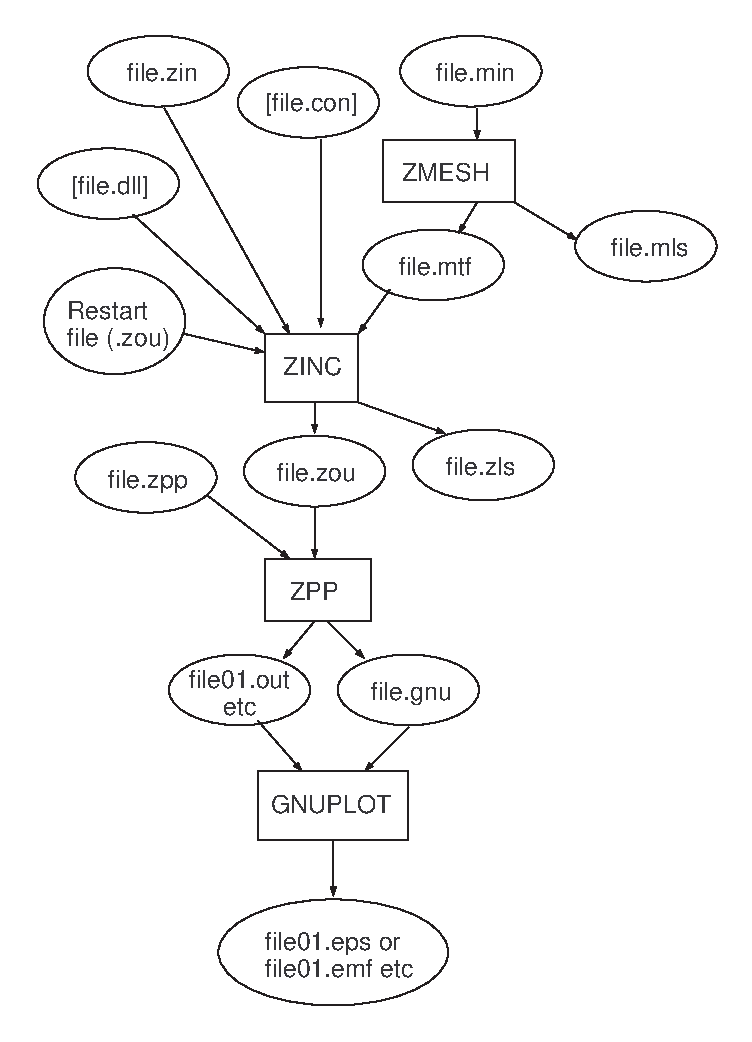
\includegraphics{zincdia}}
  \caption{The operation of \zinc. Ellipses are files and rectangles
    are programs. Optional input files are shown in [brackets]. The
    DLL file can be generated using any programming language}
  \label{zincdia}
\end{figure}

With these ideas in mind, let us look at the operation of \zinc, which
is shown diagrammatically in \f{zincdia}. This looks complex but bear
with us!  The user can choose any stem name "file" for the
simulation. Thus, \var{file.zin} might become
\var{fuelcellcathode.zin} for example. The \var{file.zin} file
contains all information about the physics of the problem to be
solved.  \var{file.con} (optional) contains a list of convenient
constants in the simulation which may be referred in
\var{file.zin}. Eg, we can store \var{eps0=8.854e-12}, the
permittivity of free space. The permittivity of a material with
rel. permittivity 2 can then be entered as \var{2*eps0} rather than
the less meaningful \var{1.778e-11}. \var{file.dll}
contains the above-mentioned non-linear functions (if needed), more
details of which are shown in \sect{nonlin}. 

Before a geometry can be solved in FE it needs to be broken up into
many small shapes called \emph{elements} through a process known as
\emph{meshing}. The \zinc\ program \zmesh\ provides this
functionalilty. The user writes \var{file.min} which specifies the
geometry in terms of primitive shapes. \zmesh\ then processes this
file to create an FE mesh and outputs \var{file.mtf} which contains
the geometry and position of all the elements.

The user than runs the core \zinc\ program which writes an output file
\var{file.zou} containing the solution on each of the FE nodes. This
file can be viewed directly using \zmesh\ but for more advanced views
and post processing, the code \zpp\ is provided. \zpp\ (\zinc\ post
processor) reads the file \var{file.zpp}, in which the user specifies
a series of linescans, plane scans, integrals etc and generates corresponding
graphs. The user can plot arbitrary expressions based on the
simulation variables and their derivatives. \zpp\ automatically plots
all files on the screen and also creates graph files in the form of
Enhanced Metafiles (EMF) or Encapsulated Postscript (EPS) files. EMF
files are convenient for Microsoft Office programs while EPS is
suitable for \LaTeX: both are vector formats.

In order to generate these graphs, \zpp\ outputs the datafiles
\var{file01.out, file02.out...} etc. These are simply numbered in
order created (depending on how many such plots the user has
requested). \zpp\ then calls Gnuplot \cite{gnuplot} (using
auto-generated command file \var{file.gnu}) to generate the graphs
needed. Since the \var{*.out} files are still left behind on disk, it
is easy to recreate the graphs when needed. The user can use Gnuplot
separately from \zinc\ to change the symbols, titles and formatting of
the graph or to plot several simulation results in one graph. One
could, for example, compare simulation results with experimental
data. Since the raw data files are always on disk there's never any
mystery about where a graph came from. This approach therefore
provides good traceability and flexiblity. See the Tutorial Manual,
Chapter 1 for more details on advanced graph plotting.

Gnuplot, by the way, is a general purpose free graph plotting program
that is bundled with the \zinc\ installation. You can use Gnuplot
independently of \zinc\ and it comes with its own manual and
tutorials.

\chapter{Installing and running Zinc}

\zinc\ is installed using an automatic installer which will guide you
through the process. The three programs, \zmesh, \zinc, \zpp, are
available to run from the Start Menu in Windows. The programs can also
be invoked from the command line as
\begin{verbatim}
  zmesh filename
  zinc filename
  zpp filename
\end{verbatim}
This latter technique is useful for running \zinc\ under batch
control. \zinc\ can also be run from external programming systems like
Matlab, Python or Excel.

The actual filenames for the \zinc\ programs are:
\begin{description}
  \item[zinc.exe] Core solver, runs at the command line.
  \item[zincwin.exe] Windows version of \zinc.
  \item[zpp.exe] Post processor, runs at the command line.
  \item[zppwin.exe] Windows version of \zpp.
  \item[zmesh.exe] Non-interactive mesh generation.
  \item[zmeshwin.exe] Interactive mesh generation/visualization package.
\end{description}

When \zinc\ installs, the Windows versions of \zmesh, \zinc, and
\zpp\ appear in the Start Menu. The installer adds \zinc's directory
to your PATH so that you can conveniently run \zinc\ from the command
prompt. Windows programs like \var{zincwin.exe} provide a simple GUI front
end to their command line equivalents, like \var{zinc.exe}.

\zinc\ also comes bundled with Gnuplot. \zpp\ invokes Gnuplot to
generate graphs. Gnuplot is then available for the user to run
independently from \zinc. Gnuplot comes with documentation and many
tutorial examples. Since \zpp\ emits text output files as well, these
can be plotted using any graph plotter or spreadsheet
program. However, we recommend the use of Gnuplot for best speed and
quality.

For advanced, non-linear operation, the user will need to prepare DLL
files for \zinc\ to link to. A free compiler like \var{gcc} or
\var{gfortran} will do (\var{http://gcc.gnu.org/wiki/GFortran}).  See
the Tutorial Manual, Chapter 3, for an example of preparing a DLL file
to link to \zinc. The user does not need to recompile \zinc.

\section{Zinc install directory}

In the install directory you will find the directory
\var{examples}. This contains several worked examples each of which is
described in the Tutorial Manual. Also there is a \var{mesh\_examples}
directory which contains various meshing examples (\var{.min}
files). You should try some of these out in \zmesh.

Other useful files include \var{nltemplate.f90, nltemplate.c} which
contain empty user specified functions for non-linear simulations. If
you are running an advanced non-linear simulation, you can create your
non-linear functions by copying these templates and filling in the
functions provided.

If you are running \zinc\ from another system like Python or Matlab,
it may be preferable to run \zinc\ and \zpp\ indirectly using the
provided batch files \var{zincrun, zpprun}. These tiny batch files
simply ensure that the \zinc, \zpp\ command prompts stay open
should an error occur. Otherwise you will not be able to read the
error before the box closes. Useage:
\begin{verbatim}
  zincrun file
  zpprun file
\end{verbatim}

\section{Uninstalling zinc}
Simply use the ``Unistall'' icon in the Start Menu. If you install a
newer version of \zinc, you should uninstall the old version
first. Note, everything in the \zinc\ install directory will be
deleted so you \emph{should not store simulation runs in the
  \zinc\ install directory}.

\section{Linux and Mac}

While \zinc\ has been written for Windows computers, it runs perfectly
on Linux and Mac using the Wine system \cite{wine}. Wine comes bundled
with most Linux systems (if not try the EPEL repository) and is
available for download on Mac, under the name
WineBottler\cite{winebottler} (free) and CrossOver\cite{crossover}
(commercial). The Wine website contains comprehensive information on
running Windows programs with Wine. To install \zinc, you should run
the installer executable through Wine. Then run \zmesh, \zinc\ and
\zpp\ through Wine. Note that Wine Is Not an Emulator (hence, WINE) so
when \zinc\ runs through Wine on Linux or Mac it should run at the
same speed as on a Windows PC with comparable hardware.

One issue we've noticed on Linux: it's better to install \zinc\ in a directory
without spaces in its path, i.e., \emph{not} in the default
\var{c:\textbackslash program files\textbackslash zinc}
directory. Similarly the directory where you store your actual
simulations should probably be free of spaces.

\section{Zinc Memory requirements}
\label{memory}

Most of \zinc's memory requirement is due to storing the FE matrix
$Q$. This is stored in sparse format in \texttt{Qval(ip), iQ(ip),
  jQ(ip), ip=1,...,lenQ} where \texttt{lenQ=nnod*nvar$^2$*27}. Here,
\var{nnod, nvar} are the total number of nodes and number of dependent
variables being solved-for respectively (e.g. in a piezoelectric
simulation \var{nvar=4} since we solve for the 3 components of elastic
displacement and also the voltage). \zinc\ uses 8 byte real numbers
(double precision) and 4 byte integers. Therefore each entry in $Q$
uses 8+4+4=16 bytes and the total memory requirement is about
\texttt{nnod*nvar$^2$*27*16} bytes. If \zinc\ cannot allocate enough
memory for the simulation it will tell you when it starts up.

\chapter{Meshing with Zmesh}
\label{zmeshchap}

Before we can simulate a problem in \zinc, the geometry must first be
meshed. This is the process of decomposing the required geometry into
small \emph{elements}. \zinc\ requires that the geometry be meshed
into \emph{hexahedral elements} and this may be accomplished by using
the included program \zmesh. A hexahedron is a six sided solid figures
resembling a squashed cube. Cuboids are special cases of hexahedrons:
if the geometry is a laminar system, for example, it may be sufficient
to use cuboid hexahedrons. In general, however, \zmesh\ will distort
the hexahedrons so as to conform to surfaces in the geometry
specified. \zmesh\ works by reading in the geometry specification from
file \var{file.min} and writing out \var{file.mtf} which contains the
shape and position of each element. \var{file.mtf} is just a text
file, whose format is described in Appendix \ref{mtfdesc}, so you can
write your own program to do the meshing if you want. This may be
useful in cases where the geometry consists of irregular shapes. For
example, we had a project to model the stress/strain of ferroelectric
domains. We wrote a program to convert the domain map output by a
microscopic imaging device into the corresponding
\var{file.mtf}. \zmesh\ would not have been helpful in this case,
since the shapes are irregular and better represented as a ``map''
rather than a series of primitive shapes like spheres and boxes.

\zmesh\ uses the same geometry specification format as
\emph{MetaMesh}, a commercial meshing program available from Field
Precision\footnote{www.fieldp.com}. As such, MetaMesh can be used in
place of \zmesh\ if required. Metamesh has many more features than
\zmesh\ including a more advanced graphical front end and the ability
to read stereo lithography (STL) and other popular CAD files for geometry
specification. Although more basic, \zmesh\ will do the job in most
systems and at least it's free! The user may want to try using
\zmesh\ first, to see whether the \zinc\ package as a whole is
suitable to his/her needs. Then, if more sophisticated geometries are
needed, the user can opt to purchase MetaMesh directly from the Field
Precision website.

\section{The Zmesh program}
\label{zmeshsec}

\begin{figure}
  \includegraphics{zmesh}
  \caption{Zmesh: a program for meshing arbitrary structures.}
  \label{zmesh}
\end{figure}

Zmesh is an interactive program as shown in \f{zmesh}. The user first
prepares an input file, \var{file.min} which contains all the geometry
details, \sect{mindesc}. He/she then uses the \verb+File > Open MIN+
command to read this file. At this point the file can be examined
using \verb+File > View MIN+. If all is well, the file can be
processed using \verb+File > Process+. A meshed geometry is then
created and is saved automatically as \var{file.mtf}. This geometry
appears on screen and can be rotated by dragging on screen (the arrow
keys can also be used). Various viewing options also exist as
described below. A pre-existing mesh file \var{file.mtf} can be read
using \verb+File > open MTF+

If you have already run a \zinc\ simulation, you can view the result
using \verb+File > open ZOU+. This shows a colour-coded view of the
data with a colour bar (on the left) indicating values. You
can cycle through the variables using the ``\verb+<+'' and ``\verb+>+''
buttons. This feature is intended to give a basic look at the raw data
solved by the simulation. For post processing, linescans and surface
plots (i.e. more quantitative information) use \zpp.

\subsection{File menu}
\begin{description}
  \item[Open MIN] read geometry input file.
  \item[Open MTF] read pre-processed mesh definition file.
  \item[Open ZOU] View a solution file. Shows a basic view of the
    data. For more advanced views and post processing, use \zpp.
  \item[Open RESID] read file showing residual distribution. Useful
    for checking solution accuracy. \zinc\ outputs this file if the
    \var{residual} command is set in the ZIN file: see \sect{zincini}.
  \item[View MIN] Show input file on screen. Note that this file
    cannot be edited. The user should use a text editor to create and edit the
    file. Notepad will do but a programming text editor may be
    preferable. We use Emacs, a free text editor with many advanced
    features. For complex geometries it may be useful to generate
    \var{file.min} using a computer program.
  \item[Process] Process the currently loaded MIN file, create the
    output MTF file and display the mesh.
  \item[Exit] Terminate the program
\end{description}

\subsection{View Menu}
\begin{description}
  \item[Bounding box] Brings up a dialog allowing user to select a
    rectangular section of the simulation volume to display. User
    selects minimum and maximum \var{i,j,k} values (indexing system
    for elements). The maximum extents allowed are shown to the right
    of the dialog. Click ``All'' to set the maximum extents and show
    the whole system. Click ``one'' to select only one element which
    is taken to be that specified by \var{imin, jmin, kmin}
  \item[Show extra] Toggle ``extra'' user-specified geometry elements
    on and off. The elements are specified in \var{file.extra} if
    present. See \sect{extra} for more details.
  \item[Distort] Normally the system geometry is shown to scale. It
    may be more convenient to distort the system for easy
    viewing. This option allows magnification factors to be entered in
    the x, y and z directions.
  \item[Show gridlines] Toggles showing the perimeters of finite
    elements. Turning gridlines off can be useful for displaying
    simulation results.
  \item[Export View] Allows you to export the current view as an
    Enhanced Metafile (EMF) (picture file).
  \item[Copy View] Copies the current view to the clipboard.
\end{description}

\subsection{On screen controls}
Drag the on screen objects with the mouse to rotate (or use arrow
keys). Zoom in/out using keys ``A'' and ``Z''. Rotate in the plane
using keys ``N'' and ``M''. Shift the view around by holding ``Shift''
and dragging with the mouse.

When it meshes a geometry, \zmesh\ assigns a \emph{region number} to
each element. The region number will later be associated with a
materials in the \var{.zin} file. Eg region 1 might be set to copper
and region 2 to aluminium. This means all elements tagged as region 1
will contain copper material. Similarly nodes are also assigned region
numbers. This is typically done to specify Dirichlet boundary
conditions. Eg we might specify that all nodes in region 1 have their
voltage set to 1 V.

A legend for the region numbers are listed on the right of the
screen. Left click to toggle a region on or off. (when a region is off
a cross appears in the box). Switching a region off just means making
it invisible. For example, in \f{zmesh}(a), region 1 has been switched
off, meaning all elements with region 1 are invisible. This allows
easier viewing of region 2 (a sphere in this case). When viewing a
simultion result file (ZOU file), these buttons have three states: on,
DATA, off. The DATA state shows colour coded data for the given region
with a colour legend on the left of the screen.

A legend for node numbers is also listed on the right of the screen
and works in the same way. You can toggle regions of nodes on or off.

Right clicking on a region or node box within the legend brings up a
colour dialog box which allows the user to change the colour for the
indicated region number.

When viewing a simulation result (ZOU file), you can ctrl-click on an
element to see the solution value at that point. The solution value is
shown in the Output window.

The buttons along the bottom are as follows
\begin{description}
  \item[x,y,z] View along the x, y or z axes.
  \item[xslice, yslice, zslice] View a slice through the system (ie a
    single plane of elements), for example as shown in \f{zmesh}(b). You can
    change which slice is displayed using the up and down arrows on
    the keyboard.
    \item[off] Switch off slices so that the whole system is displayed.
\end{description}

\subsection{Output window}
\zmesh\ gives various notifications to the user in the output
window. These include, details of meshing or any errors encountered in
the input file.

\section{Structure of the geometry input file}
\label{mindesc}

The mesh input file \var{file.min} has the form
\begin{verbatim}
  global
     <global commands>
  end

  part 1
     <part commands>
  end

  part 2
     <part commands>
  end

  :

  endfile
\end{verbatim}

\begin{figure}
  \scalebox{0.7}{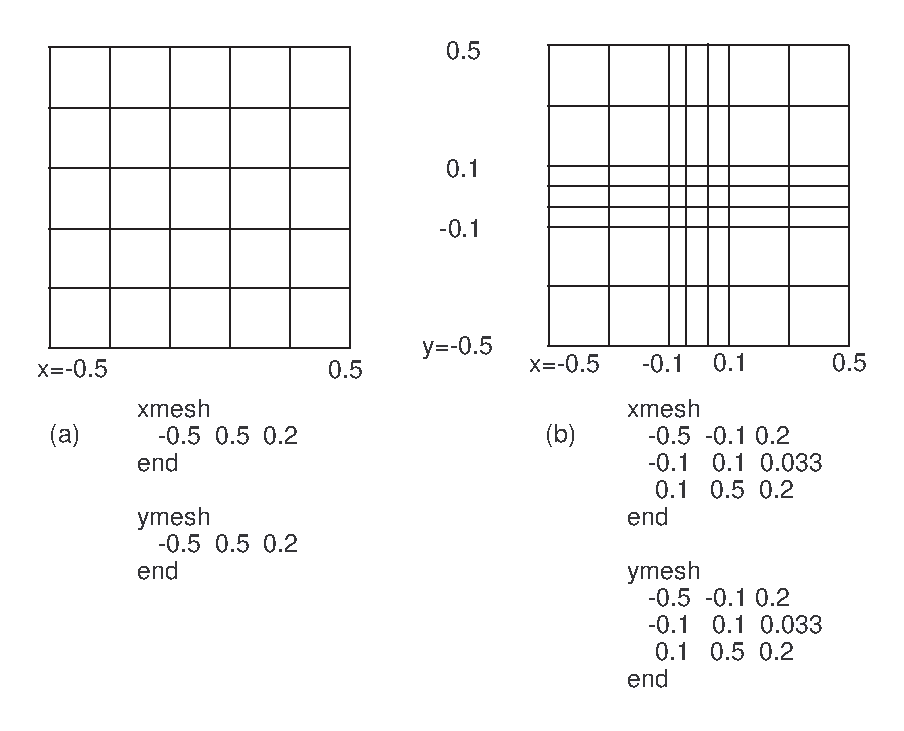
\includegraphics{logical}}
  \caption{Logical mesh formed using the global commands shown. (In the
    real file a \var{zmesh} command is also needed. For simplicity,
    these figures show a 2-D analogy). (a) Single meshing interval with
    one xmesh and one ymesh command; (b) variable meshing with
    multiple meshing commands}
  \label{logical}
\end{figure}

The global commands specifies the \emph{logical mesh} and various
global variables which define the quality of the meshing. The ``part''
commands define various shapes (spheres, cubes, extrusions etc) that
make up the geometry needed. Note that \emph{later parts overlap
  earlier ones so the order of parts is important}. The logical mesh
is illustrated in \f{logical}: it is a simple cuboid mesh defined by
the global commands \var{xmesh, ymesh, zmesh} as illustrated in that
figure. The logical mesh defines the number of elements and nodes
(intersection of the lines shown) in the simulation and also the
extent of the simulation. In \f{logical}, for example, the simulation
stretches from $-0.5$ to $0.5$ in all directions. Note that the
overall simulation area is always cuboid shaped. (However, it is
possible to model curved outer boundaries by setting the properties of
an outer region to correspond to vacuum). Distance
units are not specified at this stage, so the value 0.5 may be metres
or angstroms. In \zinc\ input file \var{file.zin} it is possible to
scale the geometry using a scale factor as required, see \sect{zinctrl}. The
global commands \var{xmesh} has the form
\begin{verbatim}
  xmesh
    x1  x2 dx1
    x2  x3 dx2
  :
  end
\end{verbatim}
where \var{[x1,x2]} is a line segment divided into intervals \var{dx1}
wide etc. If \var{xmesh} contains only one command line, the meshing
is uniform across the whole simulation region. If there are multiple
lines as in \f{logical}(b), this allows variable meshing as shown. The commands
\var{ymesh, zmesh} have exactly the same form.

\begin{figure}
  \scalebox{0.7}{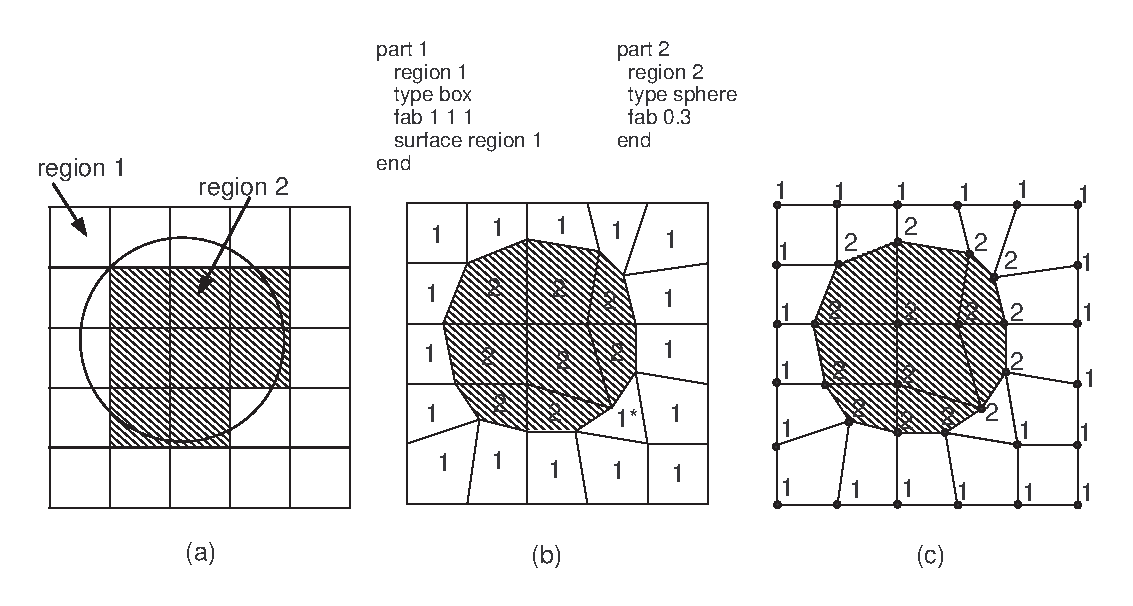
\includegraphics{meshing}}
  \caption{Meshing of two parts using the commands shown. The second
    part (sphere) is inserted into the initial box part. (a)
    Identification of element region numbers in original logical mesh;
    (b) nodes are moved onto surface between the two regions. Element
    region numbers shown. Note that the element marked (*) is not
    acceptable since it is inverted (see text). In practice, \zmesh\
    avoids inverted elements or at least gives a warning; (c) Final
    node region numbers}
  \label{meshing}
\end{figure}

\zmesh\ then processes the parts one by one as shown in \f{meshing}. In
response to the two part commands shown, a sphere is created inside a
cube. The cube is specified first and covers the whole simulation
region. Then, the sphere is specified which is inserted into the cube
(ie the cube is \emph{overwritten}. This shows the importance of parts order in
the file). Notice that the cube is designated ``region 1'' and the
sphere as ``region 2''. These region numbers will later be linked to
material properties in \var{file.zin}. \f{meshing}(a) shows what
happens in response to the part 2 command. \zmesh\ identifies the
elements whose centroids are inside the sphere specified and sets the
elements as region 2. In response to the \var{surface} command in the
part 2 'block', \zmesh\ then moves nodes so that they lie on the sphere
creating a shape which more closely conforms to the sphere. Without
the surface command, the elements would remain cuboid and the
``sphere'' would have the blocky, ``staircase'' appearance shown in
\f{meshing}(a). The final appearance and region number of each element
is shown in \f{meshing}(b). (Note that the picture shows an inverted
element which would actually be fixed by \zmesh. An inverted element
has a Jacobian which changes sign across the element preventing the
code from integrating correctly over the element (See Theoretical
Manual). \zmesh\ determines whether elements are inverted by calculating
the Jacobian. If it is inverted \zmesh\ relaxes the lattice to attempt
to fix the element even if that means having a less conforming mesh. A
chevron shaped element is considered inverted, for example)

Nodes are also given ``region numbers'' as shown in
\f{meshing}(c). This is in order to specify Dirichlet boundary
conditions \sect{regionspec} whereby field values are specified on
particular nodes. For example, in an electrostatic problem we could
designate region 2 nodes as having a fixed potential which would make
the sphere into a perfectly conducting object. The default region
numbering of nodes -- in this example -- is shown in \f{meshing}(c):
all nodes surrounding an element are given the same region number as
that element. Thus, after processing part 1, all nodes are designated
region 1. After processing part 2, the nodes within the sphere
(including those on the sphere's surface) are renumbered region
2. Note that the nodes at the interface between the two regions are
set to region 2 (since part 2 was processed last). In some cases, it
is necessary to override this behaviour and give a different region
number to the interface nodes. This can be accomplished by use of the
\var{coat} command as shown in \f{coat}(a). In this case, while
processing part 2, \zmesh\ gathers all nodes at the interface between
this part and region 1 and numbers these as region 6.

\begin{figure}
  \scalebox{0.7}{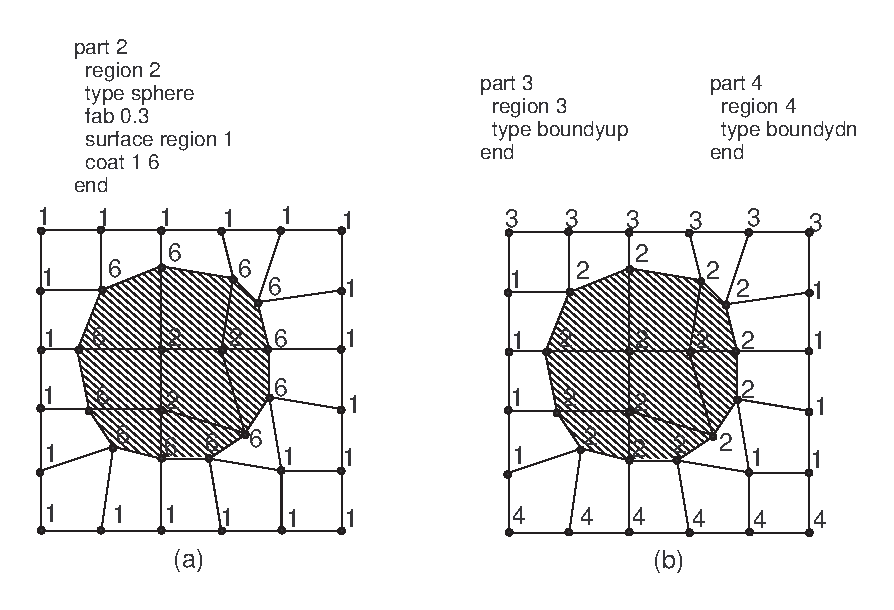
\includegraphics{coat}}
  \caption{(a) Use of the coat command to change the node region
    numbers at an interface; (b) use of open parts (\var{boundyup} and
    \var{boundydn}) to change the node region numbers}
  \label{coat}
\end{figure}

Another way to set node region numbers is to use ``open parts'' as shown
in \f{coat}(b). Here we have used two additional parts (3 and 4). These
define surfaces at the top and of the simulation whose nodes are set
to region 3 and region 4 respectively. In this example (assuming an
electrostatic problem), it would be possible to excite the system by
putting 1 V on region 3 nodes (top, Dirichlet boundary) and zero volts
on region 4 nodes (bottom, Dirichlet boundary). This would create an
electric field on the simulation. In elastic problems, this would
correspond to clamped displacements at the top and bottom of the
simulation, and so on.

\f{zintest} shows the corresponding \var{file.zin} for \f{coat} set up as an
electrostatic problem. This file will be described in more detail in
\sect{zincini} but for now note how region 1 and region 2 elements are given
permittivity values of $\epsilon_0$ (permittivity of free space,
$8.854\times10^{-12}$ F/m) and $2\epsilon_0$. Also, region 3 and
region 4 nodes are set to voltage values 1 V and 0 V
respectively. Region 1 and 2 nodes are not set at all, so these nodes
(the interior nodes in the problem) are allowed to vary in order to
solve the electrostatic equations.

\begin{figure}
\begin{verbatim}
<global commands>
:
  region 1 elements C
     V x V x = 8.854e-12
     V y V y = 8.854e-12
     V z V z = 8.854e-12
  end

  region 2 elements C
     V x V x = 1.7708e-11
     V y V y = 1.7708e-11
     V z V z = 1.7708e-11
  end

  region 3 nodes
    V=1
  end

  region 4 nodes
    V=0
  end
\end{verbatim}
\caption{Sample \zinc\ input file, \var{file.zin} corresponding to the
  setup of \f{coat}(b)}
\label{zintest}
\end{figure}

By the end of the part fitting process, all elements and nodes should
be given an region number. If this is not the case, \zmesh\ will
report an error. It is common practice for the first part to be a box
part which covers the whole simulation area. Other parts are then
inserted into this part.

We have so far described most of the part commands: \var{type, region,
  fab, surface, coat}. The other two commands are shift and rotate,
allowing the part to be shifted and rotated into the required
position. Parts are conceptually constructed at the origin $(0,0,0)$
with major axes generally along $x,y,z$. Thus, the ``box'' part is
constructed with principle axes along the x,y,z directions. It is
centred at the origin and its extents are given by the 3 numbers
following the \var{fab} (fabricate) command. The meaning of the fab
parameters depends on the part and is given in \tab{3dparts}.

The rotation command has the form
\begin{verbatim}
  rotate rx ry rz [string]
\end{verbatim}
If string is absent then a rotation is performed about the (global)
x-axis, then the y-axis then the z-axis by the angle given, in
degrees. If a different order is required, this can be given using the
string. Eg using ``yzx'' would cause rotation to occur about y, then z
then x. Since these are Euler angles, \emph{rotation order is
  important}. Furthermore, \emph{rotation is performed before the
  object is shifted} irrespective of the order of commands in the part
block.

The shift command has the form
\begin{verbatim}
  shift x y z
\end{verbatim}
and causes the part to be shifted along the displacement specified.

\section{Neuman Boundaries}
\label{neumanbc}

So far we have discussed the creation of elements and nodes and their
region numbers, which are later associated with volumetric material
properties and Dirichlet boundary conditions respectively. The other
boundary condition supported by \zinc\ is the Neuman boundary
condition. Whereas Dirichlet boundaries fix the variables being solved
for, eg, voltage, temperature, elastic displacement, Neuman boundaries
fix derivatives of these: surface charge, thermal flux, traction
respectively. These quantities may be classified as fluxes or applied
forces of some kind. These fluxes are applied at boundaries which may
be internal to the simulation or on the external surface of the
simulation. \zmesh\ does not specify such surfaces explicitly, rather
surfaces exist between volumetric regions.  For example, the curved
surface in \f{coat}(b) between region 1 and region 2 would be
identified $1-2$ giving an extra command in \f{zintest}
\begin{verbatim}
  surface 1-2 q
     V  V = 1.0
  end

  surface 1-2 g
     V = 2
  end
\end{verbatim}

\begin{figure}
  \scalebox{0.7}{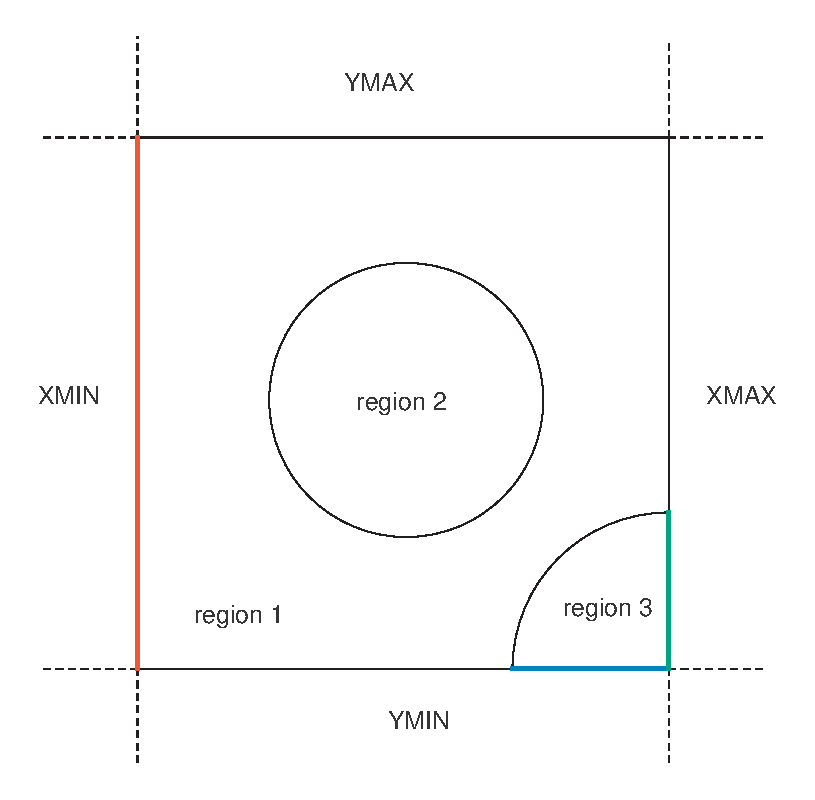
\includegraphics{outer}}
  \caption{Specification of surfaces for Neumann boundary
    conditions. Surface 1-2 is the circular surface between regions 1
    and 2. Surface 1-XMIN is the red surface, surface 3-YMIN is shown
    blue and surface 3-XMAX is shown green}
  \label{outer}
\end{figure}

The simulation is conceptually surrounded by regions called
``XMAX'', ``XMIN'', ``YMAX'', ``YMIN'', ``ZMAX'', ``ZMIN'', as shown
in \f{outer}. Thus the red outer edge on the left hand of \f{outer}
can be designated
\begin{verbatim}
  1-XMIN
\end{verbatim}
(interface between region 1 and XMIN).

\section{List of part specification commands}

There are seven (7) part specification commands which appear within a part
block (\var{part n...end}). These are: \var{type, fab, region,
  surface, coat, rotate, shift}. We have already introduced these
commands but now specify them in more detail:

\begin{description}
  \item[type] The type of part, see \tab{3dparts}. Simple parts are just of the
    form \var{type part}. Advanced parts \tab{advparts} have the form
    \verb+type <part> <Vector list> end+ with each vector on a
    separate line, \sect{advpartsec}.
  \item[fab] Fabrication info for the part. This depends on the part
    in question and is described in \tab{3dparts}, \tab{openparts},
    \tab{advparts}.
  \item[region] Elements in this part will be assigned this region
    number. Nodes around those elements will also be so assigned.
  \item[surface] This command has the form
    \verb+surface {region|part} [n] {edge} [tol]+. It causes nodes to
    be moved towards the surface between the current part and the
    specified part or region (n). This causes the mesh to conform to
    the surfaces rather than having a ``staircase'' appearance. The
    \var{edge} command causes edge fitting to take place also. If
    present, \var{tol} determines the speed of relaxation onto the
    surface. It is a number in the range 0-1. If omitted, the default
    value is 0.9 is assumed
  \item[coat] Has the form \var{coat reg regnew}. Finds all nodes at
    the interface between the current part and region \var{reg}. These
    nodes are then given region number \var{regnew}.
  \item[rotate] Has the form \verb+rotate x y z {string}+. By default,
    rotate part about the x, y and z axes in that order (angles in
    degrees). If \var{string} is present, the order of rotation may be
    altered. Eg \var{xzy} means rotate about x, then about z, then
    about y. The order of rotation is important: x,y and z are Euler
    angles. Rotation is performed before shifting.
  \item[shift] \var{shift x y z} shift the part along the vector
    specified after rotation is complete.
  \item[protect] Protects node region numbers in current part from
    being overwritten. This is useful in filled parts whose nodes
    might be overwritten by open parts. Since open parts are always
    processed \emph{after} filled parts, it is not possible to simply
    rearrange the parts order. This only affects node, not elements.
\end{description}

\section{List of global commands}

These commands must appear in the \var{global} section of the input file.

\begin{description}
  \item[xmesh, ymesh, zmesh] Specified line segments spanning the simulation
    area in the x direction. This defines the logical mesh. Each line
    segment is divided into intervals allowing variable meshing. Has
    the form \verb+xmesh <line segments> end+ with each line segment
    on a separate line of the form \var{x1 x2 dx}. Commands
    \var{ymesh, zmesh} have the same form.
  \item[presmooth N] Smooths the logical mesh using N smoothing
    steps. This is only important when variable resolution is used in
    the logical mesh. Default: no smoothing.
  \item[axissmooth dir N] Smooths along one direction ``dir''
    only. Dir is either x, y, or z. N is the number of steps. Default:
    no axis smoothing.
  \item[smooth N] Smooths the final mesh after part fitting has been
    accomplished. N steps of relaxation, default 10.
  \item[format] \verb+Format {ascii|binary}+ causes the mesh output
    file to be text (\var{file.mtf}) or binary (\var{file.mdf}) respectively.
\end{description}

\section{List of basic 3D parts}

These parts may be rotated/shifted into position using \var{rotate}
and \var{shift} commands. They are listed in \tab{3dparts}.

\begin{table}
  \begin{tabular}{lll}
    Shape & Fab parameters & Description\\\hline\hline
    \var{box} & Lx Ly Lz & Centred at origin and extends [-Lx,Lx] along x etc\\ \hline
    \var{sphere} & R & Centred at origin with radius R\\ \hline
    \var{cylinder} & R H & Centred at origin with radius R and extends [-H/2,H/2] along z\\ \hline
    \var{cone} & R H Hz & Truncated cone along $z$ with base at $z=0$ with radius R. \\
    & & Apex at $z=H$ and truncated at $z=Hz$\\ \hline
    
    \var{ellipcyl} & Rx Ry H & Cylinder along z with elliptical cross section extending \\ & &x=[-Rx,Rx], y=[-Ry,Ry]\\\hline
    \var{ellipsoid} & Rx Ry Rz & Ellipsoid given by $(x/R_x)^2+(y/R_y)^2+(z/R_z)^2=1$\\\hline
    \var{torus} & R r & R is major radius and r is minor radius. \\ & & Plane of the ``hole'' is normal to $z$\\\hline
    \var{helix} & R r H Hw & Circular cross section helix (radius r) which wraps around \\
    & & a z-directed cylinder height H, radius R centred at the origin. \\
    & & Hw is the height along z attained during 1 revolution.\\ \hline
    
    \var{trapezoid} & LxU LxD Ly Lz & Prism along z with trapezoidal cross section. \\
    & & Full width in x is LxU (top) and LxD (bottom). \\
    & & Full width in y and z given by Ly, Lz \\ \hline
  \end{tabular}

  \caption{List of 3-D parts and the meaning of the fab command for each}
\label{3dparts}
\end{table}

\section{List of open parts}
These parts have no volume so elements are not effected. The only
result is to change the region numbers of nodes. These parts are 0-D, 1-D
or 2-D shapes and may be rotated and shifted into position using \var{rotate}
and \var{shift} commands. Note that \var{boundxup} etc do not need fab
commands and are unaffected by \var{rotate} and \var{shift}. The parts
are listed in \tab{openparts}.

\begin{table}
  \begin{tabular}{lll}
    Part & fab params & Description \\ \hline\hline
    \var{point} & x y z & Creates a point at (x,y,z) \\ \hline
    \var{boundxup} & (none) & plate comprising the upper x plane of the simulation \\ \hline
    \var{boundxdn} & (none) & plate comprising the lower x plane of the simulation\\ \hline
    \var{boundyup} & (none) & plate comprising the upper y plane of the simulation \\ \hline
    \var{boundydn} & (none) & plate comprising the lower y plane of the simulation \\ \hline
    \var{boundzup} & (none) & plate comprising the upper z plane of the simulation \\ \hline
    \var{boundzdn} & (none) & plate comprising the lower z plane of the simulation \\ \hline
    \var{line} & L & line from (0,0,-L/2) to (0,0,L/2)\\ \hline
    \var{arc} & R $\theta_{min}$ $\theta_{max}$ & Arc in z=0 plane centred at origin from angle\\
    & & $\theta_{min}$ to $\theta_{min}$, radius R. $\theta=0$ is the x-axis. Angles in degrees.\\ \hline
    \var{circle} & R & open circle centred at origin radius R \\ \hline
    \var{rectangle} & Lx Ly & Open rectangle in z=0 from [-Lx,Lx] in x and [-Ly,Ly] in y\\ \hline
    \var{disk} & R & As circle but filled \\ \hline
    \var{plate} & Lx Ly & As rectangle but filled \\ \hline
    \var{bubble} & R & Spherical surface centred at origin radius R
  \end{tabular}
  \caption{List of open parts}
  \label{openparts}
\end{table}

\section{Advanced parts}
\label{advpartsec}
\zmesh\ supports 4 types of advanced parts which allow more general
shapes to be created: \var{extrusion, turning, transition} and
\var{neon}. Whereas the simple parts above have a single line ``type''
command (E.g. type sphere), these parts have a multi-line type command
of the form,
\begin{verbatim}
  type {extrusion|turning|transition|neon}
     <data lines>
     :
  end
\end{verbatim}

Apart from this, the part specification is the same and \var{region,
  surface, coat, shift, rotate} commands may be used as usual.

\subsection{Extrusion}

An extrusion is a prism shape along the z axis. The cross section is
built up using an arbitrary number of line or arc segments which must
form a closed 2-d shape in the x-y plane.

The \var{type} command has the form
\begin{verbatim}
  type extrusion {sidefit}
     Vector 1 {S|SE}
     Vector 2 {S|SE}
     :
  end
\end{verbatim}
Each vector describes a line or arc in the x-y plane and is of the form
\begin{verbatim}
  {L|A} xstart ystart xend yend {xcentre ycentre}
\end{verbatim}
Here, ``L'' means line and ``A'' means arc. The \var{xcentre ycentre}
specification is only required for arcs. The line extends
from \var{(xstart,ystart)} to \var{(xend,yend)} with arc centre (in
the case of arcs) at \var{(xcentre,ycentre)}. Vectors should link to
one another in sequence and form a closed loop in the x-y plane. Eg to
make a square use
\begin{verbatim}
  type extrusion
   L  0 0   1 0
   L  1 0   1 1
   L  1 1   0 1
   L  0 1   0 0
  end
\end{verbatim}
To make a circle, we could adapt this to read
\begin{verbatim}
  type extrusion
   A  0 0  1 0  0.5 0.5
   A  1 0  1 1  0.5 0.5
   A  1 1  0 1  0.5 0.5
   A  0 1  0 0  0.5 0.5
  end
\end{verbatim}
Note that \emph{arc segments may not be more the 90 degrees}. Longer
arcs should be divided into smaller ones just as we have done here.

The extrusion fab command takes a single parameter: the length of the
extrusion. 
\begin{verbatim}
  fab L
\end{verbatim}
The extrusion is along the z axis from -L/2 to L/2. The
whole extrusion can be rotated and shifted into place in the usual
way.

The optional S and SE commands at the end of each vector determine how surface
fitting is done on the extruded surface of the shape. If S is present,
the segment is surface fitted. If SE is present edge fitting is done
also. Such surface fitting is performed only if a \var{surface}
command appears in the part specification. The top and bottom part of
the surface is always fitted if such a surface command is present. To
turn off this fitting, use the \var{sidefit} specifier.

A complete part specification for extrusion looks like, for example,
\begin{verbatim}
part 1
  region 1
  type extrusion
   L  -1 0   1 0
   A   1 0   0 1   0 0
   A   0 1  -1 0   0 0
  end  
  fab 1
  rotate 90 0 0
  shift 1.0 0.0 0.0
end
\end{verbatim}
This creates prism of semi-circular cross section, length 1 along the
z axis, then rotates it around x so it now points along y. The part is
shifted so that its centre is at (1,0,0).

\subsection{Turning}
A turning part is made by constructing a 2-D shape in (r,z) plane then
rotating about the z-axis. The type command has exactly the same form
as for the extrusion (including the use of lines or arcs and the S/SE
commands):
\begin{verbatim}
  type turning {sidefit}
     Vector 1 {S|SE}
     Vector 2 {S|SE}
     :
  end
\end{verbatim}

The fab command has the form
\begin{verbatim}
  fab angmin angmax
\end{verbatim}
where \var{angmin, angmax} are the minimum and maximum turning angles
(about the z axis) in degrees. Use 0 and 360 to produce a full
turning. If the angle difference is less than 360 the turning will
have ``start'' and ``end'' faces which are fitted according to the surface
command (unless \var{sidefit} is specified). The turning may be shifted and
rotated in the usual way.

\subsection{Transition}

The transition shape consists of two planar shapes at z=zmin and
z=zmax connected together. As we go from zmin to zmax, the shape
smoothly ``morphs'' between the two shapes. The type command has the form
\begin{verbatim}
  type transition {sidefit}
    Vector 1a  Vector 1b  {S}
    Vector 2a  Vector 2b  {S}
    :
  end
\end{verbatim}
Each vector is of the form
\begin{verbatim}
  xstart ystart xend yend
\end{verbatim}
Note that arcs are not allowed so there is no need for the L or A
specification. Vector 1a (on the bottom surface) morphs into vector 1b
(on the top surface) etc. The ``S'' parameter, if present, indicates
that surface fitting will be done. The fab command has the form
\begin{verbatim}
  fab L
\end{verbatim}
The shape then extends along the z axis from z=-L/2 to z=L/2.

\subsection{Neon}
The neon shape is an arbitrary tube of circular cross section. The trajectory of the cross section is given
by a series of points:
\begin{verbatim}
  part neon
    x1 y1 z1
    x2 y2 z2
    :
  end
\end{verbatim}
where (x1,y1,z1) etc are points in 3-D space. The fab command has the form
\begin{verbatim}
  fab r
\end{verbatim}
where r is the radius of the tube.

\subsection{Summary of advanced shapes}

The advanced shapes are summarised in \tab{advparts}.

\begin{table}
\begin{tabular}{llll}
type & \var{type} command & \var{fab} & Description \\ \hline\hline
  \var{extrusion} & type extrusion \{sidefit\} & L & extrusion from z=-L/2 to z=L/2\\
& [Vector list] & \\
& end & \\ \hline
%%%%%%%%%%%%%%%%%%%%%%%%%%%%%%%%%%%%%%%%%%%%%%%%%%%%%%%%%%%%%%%%%%%%%%
  \var{turning} & type turning \{sidefit\} & $\theta_1$ $\theta_2$ & turning about z from $\theta_1$ to $\theta_2$ ($^\circ$)\\
& [Vector list] & \\
& end & \\ \hline
%%%%%%%%%%%%%%%%%%%%%%%%%%%%%%%%%%%%%%%%%%%%%%%%%%%%%%%%%%%%%%%%%%%%%%
  \var{transition} & type transition \{sidefit\} & L & transition along z from z=-L/2 to L/2\\
& [Vector pair list] & \\
& end & \\ \hline
%%%%%%%%%%%%%%%%%%%%%%%%%%%%%%%%%%%%%%%%%%%%%%%%%%%%%%%%%%%%%%%%%%%%%%
  \var{neon} & type neon & r & Circular tube radius r \\
& [points list] & \\
& end & \\ \hline
\end{tabular}  
  \caption{Table of advanced shapes. A Vector has the form \var{xstart
      ystart xend yend \{xcentre ycentre\} \{S|SE\}}. A Vector pair
    has the form \var{xstarta ystarta xstartb ystartb \{S\}}}
\label{advparts}
\end{table}

\section{User specified graphics (optional)}
\label{extra}

\begin{figure}
  \scalebox{0.5}{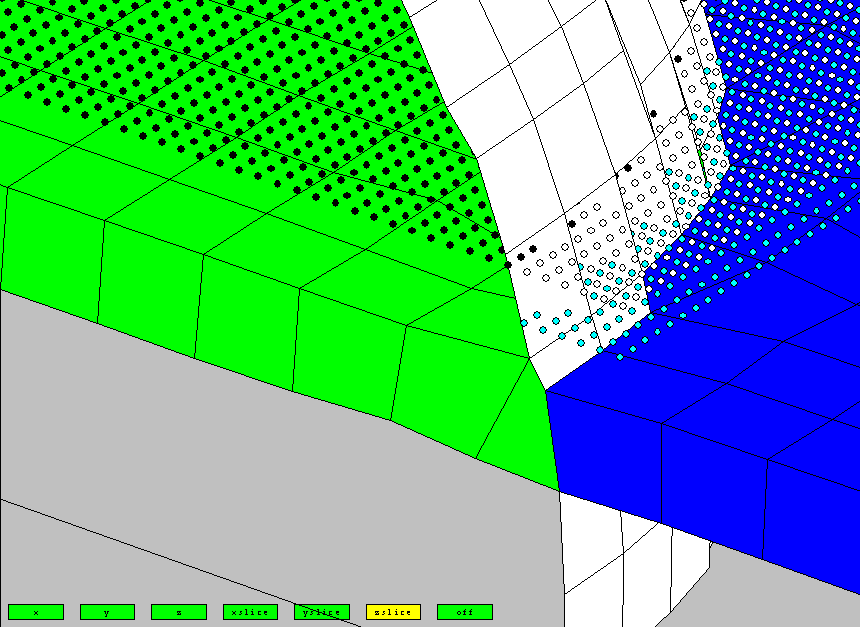
\includegraphics{extrapic}}
  \caption{Zmesh view with additional user specified graphics: black,
    white, cyan dots and white quadrilaterals}
  \label{extrapic}
\end{figure}

In addition showing the meshing (nodes and elements) of a simulation,
the user can also add additional graphics to the view. For example,
\f{extrapic} shows a Zmesh view for a hybrid model we have been
working on. In this model, atoms are present as well as finite
elements. In \f{extrapic}, we see the positions of the atoms (black,
white and blue symbols) and the surface of interactions netween the
atomic and FE regions (white polygons). The green and dark blue
hexahedra are simply Zmesh's usual output. The additional graphics
have been specified in a file \var{file.extra}. When loading
\var{file.mtf}, Zmesh also loads \var{file.extra} if it exists. This
file consists of any number of lines each of which specifies one of
the supported user graphics: currently either a point in space (type
1), or a quadrilateral (type 2). \emph{Points} have the form
\begin{verbatim}
  1  x y z r g b
\end{verbatim}
where $(x,y,z)$ is the position in space (using the usual simulation
coordinate system) and \var{r,g,b} give the red, green and blue
specification of the colour for the point. These numbers must be in
the range [0,255]. For example (r=255, g=0, b=0) gives
red. \emph{Quadrilaterals} have the form
\begin{verbatim}
  2  x1 y1 z1  x2 y2 z2  x3 y3 z3  x4 y4 z4 r g b
\end{verbatim}
where $(x_1,y_1,z_1)$ etc are the vertices of the quadrilateral which
should be specified in order (clockwise or anticlockwise) and
\var{r,g,b} give the colour specification for the quadrilateral.

The user can specify any number of graphical elements, however, the
maximum number of \emph{different} colours which can be specified is 100.

The user specified graphics can be switched on and off using the
``Show extra'' command in the View menu.

\chapter{PDE specification}

\section{Static problems}
\label{pdestatic}

For static systems, \zinc\ supports the following partial differential
equation sets
\begin{eqnarray}
  -\div \vec C\grad\vec u+\vec a\vec u&=&\vec f \label{voleq}\\
  \vec n\cdot \vec C\grad\vec u+q\vec u&=&\vec g,~~ \t{(Neumann~boundary~condition)} \label{neu}
\end{eqnarray}
Here $\vec u=(u_1,u_2,...)$ where $u_1(x,y,z)$ etc are the independent
variables to be solved for. For example $u_1$ might be electrostatic
potential and $u_2$ temperature (as in the example of
\sect{thermo}). One must set the various components of \caf, \qg\ so that,
when \eq{voleq} is multiplied out, we obtain the needed set of PDEs
and boundary conditions. Here, the meaning of grad and div is
non-standard. For example, with two variables, we define
\begin{eqnarray}
  \grad\vec u = (\grad u_1,\grad u_2)\\
  \div (\vec a | \vec b)=(\div\vec a, \div\vec b)
\end{eqnarray}
where $(\vec a | \vec b)$ is a 6-vector (in 3D space) partitioned into
two, 3-vectors. Thus, grad is applied to each element in $\vec u$ and
div takes groups of three variables and compacts them into one.

\begin{figure}
  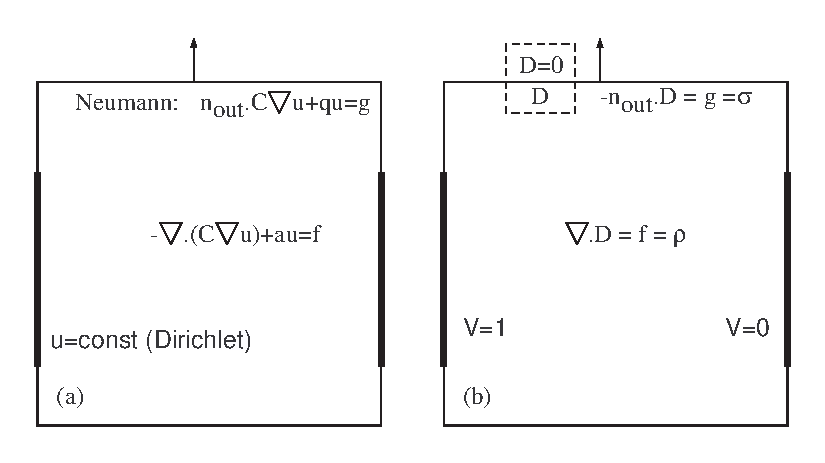
\includegraphics{Dboundary}
  \caption{(a) Bulk PDE and boundary condition specification; (b)
    Electrostatic example. The dashed box is a Gaussian surface (see
    text)}
  \label{Dboundary}
\end{figure}

Equation \eq{voleq} applies within the bulk of the system and \eq{neu}
applies on the simulation surfaces as shown in
\f{Dboundary}(a). However if a \emph{Dirichlet} boundary is applied
(simply setting the solved-for variables to a constant) then Neuman
boundaries are deactivated at that point. \f{Dboundary}(b) shows a
specific example where $C$ is set to the permittivity tensor (more
specific details in \sect{thermo}, \sect{multiferroic}) giving an
electrostatic problem. In this case, using $a=q=0$ the bulk PDE
becomes $\div \vec D=f$ where the Zinc parameter $f$ is evidentally equal
to the volumetric charge $\rho$. On the surface, the Neumann boundary
becomes $-\vec n\cdot\vec D=g$ as shown in \f{Dboundary}(b). If we
construct a Gaussian surface as shown in the figure, it is clear that
this is just equal to the surface charge $\sigma$, so we conclude that
$g=\sigma$ in this example. If we set $g=0$ on the surface, in this
example, the boundary condition becomes, simply $-\vec n\cdot\vec D=0$
a typical ``open boundary'' used in electrostatic problems. In \zinc,
any parameter \caf, \qg\ \emph{which is not set defaults to zero}, so if you
don't set $g$ at all you will get this open boundary everywhere you
haven't set Dirichlet boundaries.

All the above remarks apply equally to elastic problems: if $C$ is set
to the stiffness tensor, then $f$ will be the volume force and $\vec
g$ will be the traction on the surface (basically the applied
pressure). Setting $\vec g=0$ gives an open boundary while setting
$\vec u$ to constant value clamps the system in the specified places.

These equations can also be written in component form as
\begin{eqnarray}
    -\sum_{j=1}^3\sum_{k=1}^N\sum_{l=1}^3
\frac{\d}{\d x_j}\left(C_{ijkl} \frac{\d u_k}{\d x_l}\right)
+\sum_{k=1}^N a_{ik}u_k=f_i,~~~i=1,\ldots,N\\
  \sum_{j=1}^3\sum_{k=1}^N\sum_{l=1}^3 n_j 
\left(C_{ijkl} \frac{\d u_k}{\d x_l}\right)
+\sum_{k=1}^N q_{ik}u_k=g_i,~~\t{Neumann}~~~i=1,\ldots,N
\end{eqnarray}
where $N$ is the number of independent variables to be solved. This
general PDE specification allows a wide range of systems to be solved
including those mentioned in the introduction.

The components of \caf, \qg\ all vary in space. When the system is meshed,
it is divided into a structured mesh of \emph{hexahedral} elements
each of which is assigned a \emph{region number}. The mesh is
specified in the input file \var{filename.mtf} (see \sect{mtf}). The materials file
\var{filename.zin} specifies \caf, \qg\ values for each region, thus specifying
material properties (such as permittivity in the above example) for
each element.

The values of \caf, \qg\ components may be set to constant values or set to
vary depending on the local values of the $\vec u$ vector. In
the latter case, the problem becomes non-linear \sect{nonlin}. For
example, the components might be temperature dependent in a thermal problem. 

Comsol implements a similar set of equations: these are described in
Appendix \ref{comcoef}. A problem set in \zinc\ may easily be
converted to Comsol and vice versa.

\section{Transient problems}

\zinc\ can solve transient problems of the form
\begin{eqnarray}
  \frac{\d\vec u}{\d t}&=&\div \vec C\grad\vec u-\vec a\vec u+\vec f\\
  \vec n\cdot \vec C\grad\vec u+\vec q\vec u&=&\vec g,~~ \t{(Neumann)}
\end{eqnarray}
or, in component format
\begin{eqnarray}
  \frac{\d u_i}{\d t}=\sum_{jkl}\frac{\d}{\d x_j}\left(C_{ijkl} \frac{\d u_k}{\d x_l}\right)-a_{ik}u_k+f_i,~~~i=1,2,..,N\\
  \sum_{jkl}n_j \left(C_{ijkl} \frac{\d u_k}{\d x_l}\right)+g_{ik} u_k=g_i,~~\t{Neumann}~~~i=1,\ldots,N
\end{eqnarray}
Note that the boundary conditions are the same as in the static
case. Again, one can set up either linear or non-linear problems. All
observations about the meaning of parameters \caf, \qg\ given in
\sect{pdestatic} apply here also.

\section{Static and steady state problems}

The static mode of \zinc\ can be made to solve steady state problems
as well. Consider the problem where the $\vec u$ variables depend on
time as
\begin{equation}
  u(\vec r,t)=Re [u_\omega(\vec r) \exp(j\omega t)]
  \label{phasor}
\end{equation}
In that case we replace $\d/\d t$ with $j\omega t$ in the PDEs and the
problem again becomes spatial but we are solving for the
\emph{phasors} $u_\omega(\vec r)$. These phasors are complex numbers
whose modulus indicates time-oscillation amplitude and whose phase
gives a phase shift according to \eq{phasor}. However, \zinc\ does not
support complex variables so it will be necessary to write
$u=u_r+ju_i$ and expand each complex equation in terms of two real
equations.

Some harmonic problems give real solutions, for example if
the material properties are real (lossless). In that case
$u_\omega(\vec r)$ gives amplitudes of oscillation with each point
oscillating in phase.

\section{Internal boundaries}

\emph{This section is considered advanced and may be skipped on first reading}

In simulation problems we often have the case that material properties
vary suddenly within the simulation area giving a sharp internal
boundary. For example, we might have a sphere of PTFE
($\epsilon_r=2.1$) embedded in a cube of glass ($\epsilon_r=4.7$). At
the sharp boundary between these two layers, certain continuity
conditions are expected to be satisfied. In the electrostatic problem
just given, for instance, the normal component of the D-field
(electric displacement field) is continuous across the surface. This
continuity is a consequence of the bulk PDE specified $\eq{voleq}$,
and \zinc\ therefore includes it automatically. However, there are
cases when we want to apply discontinuities at such internal
interfaces. Continuing our example, we could place a surface charge on
the PTFE-glass interface of 1 C/m$^2$. In that case, the normal
component of the D-field is not continuous but discontinuous by an
amount equal to the surface charge applied. We now wish to formalise
this statement.

\begin{figure}
  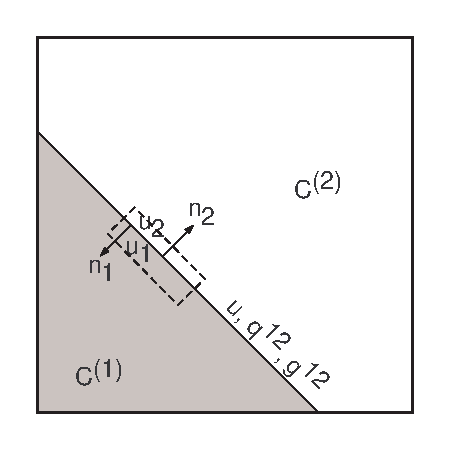
\includegraphics{continuity}
  \caption{Continuity conditions over surface 1-2. Note that $u_1$ and
    $u_2$ are defined on the surface coming from either region. In
    fact $u_1=u_2=u$: we distinguish between them because we need
    derivatives of $u_1$ and $u_2$ which differ. The dashed box is a
    Gaussian surface (see text)}
  \label{contpic}
\end{figure}

At every surface, the internal boundary is set as follows (see
\f{contpic})
\begin{eqnarray}
  -\vec n_1\cdot C^1\grad \vec u_1- \vec n_2\cdot C^2\grad \vec u_2+q^{12}\vec u=g^{12}
\label{continuity}
\end{eqnarray}
where $n_1$ and $n_2$ are the unit normals at the surface pointing
into regions 1 and 2 respectively. If $g=q=0$ then this reduces to
\begin{eqnarray}
  -\vec n_1\cdot C^1\grad \vec u_1- \vec n_2\cdot C^2\grad \vec u_2=0
\end{eqnarray}
writing $\vec n_2=-\vec n_1$ gives
\begin{eqnarray}
  \vec n_1\cdot C^1\grad \vec u_1= \vec n_1\cdot C^2\grad \vec u_2
\label{natcont}
\end{eqnarray}
which is the default continuity equation we expect if q and g are left
at zero (default values). For example, in the electrostatic problem,
we would set $C$ to the permittivity matrix and \eq{natcont}
becomes
\begin{eqnarray}
  \vec n\cdot\vec D_1=\vec n\cdot\vec D_2
\end{eqnarray}
as expected.

As discussed earlier, when you do not set something in \zinc, it
defaults to zero. So if no \var{surface} commands are included in the
\zinc\ input file, $q=g=0$ everywhere and the ``natural'' continuity
condition \eq{natcont} applies. If we \emph{do} set explicit
\var{surface}s, then we can impose specific discontinuity as in
\eq{continuity}. This facility is likely to be only rarely used as we
cannot (normally) impose internal charges/forces in real experimental
systems. Let us consider the consequences of \eq{continuity} for an
electrostatic example. Setting the C-matrix to be the permittivity,
\eq{continuity} becomes
\begin{eqnarray}
\vec n_1\cdot\vec D_1 +\vec n_2\cdot\vec D_2 = g^{12}
\end{eqnarray}
Drawing a Gaussian surface over the interface as shown in \f{contpic}
shows that
\begin{eqnarray}
  \vec n_1\cdot\vec D_1 +\vec n_2\cdot\vec D_2 = \sigma
\end{eqnarray}
so that $g^{12}=\sigma$, the applied surface charge (an observation we
already made in \sect{pdestatic}). This proves the statement made at
the start of this section that normal D-field is discontinuous
according to the surface charge. But here we have made the relation
explicit.

To give a surface charge of +1 C/m$^2$ in \f{contpic}, we would need a
surface command of the form
\begin{verbatim}
  surface 1-2 q
    V = 1.0
  end
\end{verbatim}
Note that Neumann \var{surface} commands have already been mentioned
in \sect{neumanbc} and their precise format is given in
\sect{neumanspec}

\section{Example with thermal-electrical coupling}
\label{thermo}

A simple example of how to set the matrices is an electrical
conduction/thermal system. In this case we have
\begin{eqnarray}
-\div(\vecc\sigma\grad V)=
-\frac{\d}{\d x}\left(\sigma_{11} \frac{\d V}{\d x}\right)
-\frac{\d}{\d y}\left(\sigma_{22} \frac{\d V}{\d y}\right)
-\frac{\d}{\d z}\left(\sigma_{33} \frac{\d V}{\d z}\right)=0\\
-\div(k\grad T)=
-\frac{\d}{\d x}\left(k \frac{\d T}{\d x}\right)
-\frac{\d}{\d y}\left(k \frac{\d T}{\d y}\right)
-\frac{\d}{\d z}\left(k \frac{\d T}{\d z}\right)=Q
\end{eqnarray}
where $V$ is the electric potential, $\sigma_{ij}$ is the conductivity
tensor, $T$ is temperature, $k$ is thermal conductivity, $Q$ is heat
source. These equations follow directly
from Maxwell's equation and the diffusion equation. In this case,
\begin{equation}
  \vec u=
  \left(\begin{array}{c}
    V\\
    T
  \end{array}\right)
\end{equation}

\begin{equation}
  C=
  \left(\begin{array}{ccc|ccc}
    \sigma_{11} & 0 & 0 & 0 & 0 & 0\\
    0 & \sigma_{22} & 0 & 0 & 0 & 0\\
    0 & 0 & \sigma_{33} & 0 & 0 & 0\\ \hline
    0 & 0 & 0 & k & 0 & 0\\
    0 & 0 & 0 & 0 & k & 0\\
    0 & 0 & 0 & 0 & 0 & k
  \end{array}\right)
  \label{Cthermo}
\end{equation}
We have
\begin{equation}
  \grad\vec u =
  \left(\begin{array}{c}
    \grad V\\
    \grad T
  \end{array}\right)
=
  \left(\begin{array}{c}
    \d V/\d x\\
    \d V/\d y\\
    \d V/\d z\\ \hline
    \d T/\d x\\
    \d T/\d y\\
    \d T/\d z
  \end{array}\right)
\end{equation}
so that $\div(-C\grad\vec u)$ is
\begin{equation}
  \left(\begin{array}{l}
      -\frac{\d}{\d x}(\sigma_{11} \frac{\d V}{\d x})
      -\frac{\d}{\d y}(\sigma_{22} \frac{\d V}{\d y})
      -\frac{\d}{\d z}(\sigma_{33} \frac{\d V}{\d z})\\
      -\frac{\d}{\d x}(k \frac{\d T}{\d x})
      -\frac{\d}{\d y}(k \frac{\d T}{\d y})
      -\frac{\d}{\d z}(k \frac{\d T}{\d z})
  \end{array}\right)
\end{equation}
We set $\vec f=(0,Q)$ and $\vec
a=0$ to complete the equation set needed. The Neumann BCs are, with \qg=0 of the form
\begin{eqnarray}
  n_x\sigma_{11} \frac{\d V}{\d x}+n_y\sigma_{22} \frac{\d V}{\d y}
+n_z\sigma_{33} \frac{\d V}{\d z}=0 \label{Vneu}\\
  n_x k \frac{\d T}{\d x}+n_y k \frac{\d T}{\d y}+n_z k \frac{\d T}{\d z}=0 \label{Tneu}
\end{eqnarray}
which are open or natural boundaries.

The \zinc\ C-matrix given above would be entered in the \var{.zin} file like this:
\begin{verbatim}
region 1 elements C
   1 1 = [sig11, 0, 0, &
          0, sig22, 0, &
          0, 0, sig33]

   2 2 = [k, 0, 0, &
          0, k, 0, &
          0, 0, k]
end
\end{verbatim}
assuming that \var{sig11} etc have been defined in the
\zinc\ constants (\var{.con}) file. Here ``1 1'' refers to the top
left block of the matrix and ``2 2'' to the bottom right block. The
other blocks needn't be specified as they are zero. The blocks are
always $3\times3$ in size since we model 3-D space. This specification
applies to region 1. If other regions are present we would need to
specify each region in turn in the same way. More details of
specifying \zinc\ matrices is given in \sect{regionspec}.

It may be noted that there is no
coupling between $V$ and $T$ in this problem. In fact we could have
just solved for $V$ and $T$ separately. Coupling could be introduced
by putting some non-zero off diagonals in \eq{Cthermo} or by
introducing \emph{non-linearity}. For example, the conductivities
$\sigma_{11}$ etc might depend on temperature while the heat source
$Q$ might depend on electric field (eg $Q\sim E^2$). \zinc\ can solve
non-linear problems such as this. In linear problems we must set all
the components of \caf, \qg\ to literal constants in the input files
(or expressions that evaluate to constants, see
\sect{expressions}). In non-linear problems we can set some or all of
the components to expressions involving the dependent variables. See
\sect{nonlin}.

\section{Multiferroic equations: a more complex example}
\label{multiferroic}

In multiferroics, frequency domain ($\d/\d t\to j\omega$) we may write
the equations of motion as
\begin{eqnarray}
  \sum_{j=1}^3 \frac{\d \sigma_{ij}}{\d x_j}+p_i&=&-\rho\omega^2 u_i,~~~i=1,2,3 \label{sigeq}\\
  \div\vec D&=&0 \label{Deq}\\
  \div\vec B&=&0 \label{Beq}\\
  \curl\vec E&=&0 \label{Eeq}\\
  \curl\vec H&=&0 \label{Heq}
\end{eqnarray}
These equations assume no space charge and no current. In this case we can introduce
\begin{eqnarray}
  \vec E=-\grad V \label{V}\\
  \vec H=-\grad V_m \label{Vm}\\
  \epsilon_{ij}=\frac12\left(\frac{\d u_i}{\d x_j}+\frac{\d u_j}{\d x_i}\right)\label{u}
\end{eqnarray}
so that the curl equations \eq{Eeq}, \eq{Heq} are automatically satisfied. We use linear
constitutive laws as
\begin{eqnarray}
  \sigma_{ij}=c^{EH}_{ijkl}\epsilon_{kl}-e_{kij}E_k-e_{kij}^m H_k \label{sigcon}\\
  D_i=e_{ijk}\epsilon_{jk}+\kappa_{ij}^{\epsilon H} E_j+\alpha_{ij}H_{j} \label{Dcon}\\
  B_i=e_{ijk}^m\epsilon_{jk}+\alpha_{ji}E_j+\mu_{ij}^{\epsilon E} H_j \label{Bcon}
\end{eqnarray}
with implied summation over repeated indices. The equations can be
written in matrix form as
\begin{equation}
  \left(\begin{array}{c}
    \vecc\sigma\\
    \vec D\\
    \vec B
  \end{array}\right)
=
\left(\begin{array}{ccc}
  c^{EH} & -e^T & -(e^m)^T \\
  e & \kappa^{\epsilon H} & \alpha\\
  e^m & \alpha^T & \mu^{\epsilon E}
\end{array}\right)
\left(\begin{array}{c}
  \vecc\epsilon\\
  \vec E\\
  \vec H
\end{array}\right)
\end{equation}
Substituting \eq{sigcon}-\eq{Bcon} in \eq{sigeq}-\eq{Beq} and using
\eq{V}-\eq{u}, we obtain 5 PDEs (with implied summation):
\begin{eqnarray}
\frac{\d}{\d x_j}\left[c_{ijkl}^{EH}\frac{\d u_{k}}{\d x_l}
+e_{kij}\frac{\d V}{\d x_k}+e^m_{kij}\frac{\d V_m}{\d x_k}\right]+p_i
&=&-\rho \omega^2 u_i~~~i=1,2,3 \nonumber\\
\frac{\d}{\d x_i}\left[e  _{ijk}\frac{\d u_j}{\d x_k}-\kappa^{\epsilon,H}_{ij} \frac{\d V}{\d x_j}-\alpha_{ij}\frac{\d V_m}{\d x_j}\right]&=&0 \nonumber \\
\frac{\d}{\d x_i}\left[e^m_{ijk}\frac{\d u_j}{\d x_k}-\alpha_{ji} \frac{\d V}{\d x_j}-\mu^{\epsilon,E}_{ij}\frac{\d V_m}{\d x_j}\right]&=&0 \label{multipde}
\end{eqnarray}
where the terms arising from the two components of strain in \eq{u}
are equal so that the factor of 1/2 disappears.  To input these in
\zinc, we use the following $C$ matrix (omitting some superscripts for
clarity)
\begin{equation}
  \left[\begin{array}{ccccccccc|ccc|ccc}
c_{11}  &c_{16}  &c_{15}  &c_{16}  &c_{12}  &c_{14}  &c_{15}  &c_{14}  &c_{13}  &e_{11}  &e_{21}  &e_{31}  &e^m_{11}  &e^m_{21}  &e^m_{31}  \\
c_{61}  &c_{66}  &c_{65}  &c_{66}  &c_{62}  &c_{64}  &c_{65}  &c_{64}  &c_{63}  &e_{16}  &e_{26}  &e_{36}  &e^m_{16}  &e^m_{26}  &e^m_{36}  \\
c_{51}  &c_{56}  &c_{55}  &c_{56}  &c_{52}  &c_{54}  &c_{55}  &c_{54}  &c_{53}  &e_{15}  &e_{25}  &e_{35}  &e^m_{15}  &e^m_{25}  &e^m_{35}  \\
c_{61}  &c_{66}  &c_{65}  &c_{66}  &c_{62}  &c_{64}  &c_{65}  &c_{64}  &c_{63}  &e_{16}  &e_{26}  &e_{36}  &e^m_{16}  &e^m_{26}  &e^m_{36}  \\
c_{21}  &c_{26}  &c_{25}  &c_{26}  &c_{22}  &c_{24}  &c_{25}  &c_{24}  &c_{23}  &e_{12}  &e_{22}  &e_{32}  &e^m_{12}  &e^m_{22}  &e^m_{32}  \\
c_{41}  &c_{46}  &c_{45}  &c_{46}  &c_{42}  &c_{44}  &c_{45}  &c_{44}  &c_{43}  &e_{14}  &e_{24}  &e_{34}  &e^m_{14}  &e^m_{24}  &e^m_{34}  \\
c_{51}  &c_{56}  &c_{55}  &c_{56}  &c_{52}  &c_{54}  &c_{55}  &c_{54}  &c_{53}  &e_{15}  &e_{25}  &e_{35}  &e^m_{15}  &e^m_{25}  &e^m_{35}  \\
c_{41}  &c_{46}  &c_{45}  &c_{46}  &c_{42}  &c_{44}  &c_{45}  &c_{44}  &c_{43}  &e_{14}  &e_{24}  &e_{34}  &e^m_{14}  &e^m_{24}  &e^m_{34}  \\
c_{31}  &c_{36}  &c_{35}  &c_{36}  &c_{32}  &c_{34}  &c_{35}  &c_{34}  &c_{33}  &e_{13}  &e_{23}  &e_{33}  &e^m_{13}  &e^m_{23}  &e^m_{33}  \\ \hline
e_{11}  &e_{16}  &e_{15}  &e_{16}  &e_{12}  &e_{14}  &e_{15}  &e_{14}  &e_{13}  &-\kappa_{11} &-\kappa_{12} &-\kappa_{13} &-\alpha_{11} &-\alpha_{12} &-\alpha_{13} \\
e_{21}  &e_{26}  &e_{25}  &e_{26}  &e_{22}  &e_{24}  &e_{25}  &e_{24}  &e_{23}  &-\kappa_{21} &-\kappa_{22} &-\kappa_{23} &-\alpha_{21} &-\alpha_{22} &-\alpha_{23} \\
e_{31}  &e_{36}  &e_{35}  &e_{36}  &e_{32}  &e_{34}  &e_{35}  &e_{34}  &e_{33}  &-\kappa_{31} &-\kappa_{32} &-\kappa_{33} &-\alpha_{31} &-\alpha_{32} &-\alpha_{33} \\ \hline
e^m_{11}  &e^m_{16}  &e^m_{15}  &e^m_{16}  &e^m_{12}  &e^m_{14}  &e^m_{15}  &e^m_{14}  &e^m_{13}  &-\alpha_{11} &-\alpha_{21} &-\alpha_{31} &-\mu_{11} &-\mu_{12} &-\mu_{13} \\
e^m_{21}  &e^m_{26}  &e^m_{25}  &e^m_{26}  &e^m_{22}  &e^m_{24}  &e^m_{25}  &e^m_{24}  &e^m_{23}  &-\alpha_{12} &-\alpha_{22} &-\alpha_{32} &-\mu_{21} &-\mu_{22} &-\mu_{23} \\
e^m_{31}  &e^m_{36}  &e^m_{35}  &e^m_{36}  &e^m_{32}  &e^m_{34}  &e^m_{35}  &e^m_{34}  &e^m_{33}  &-\alpha_{13} &-\alpha_{23} &-\alpha_{33} &-\mu_{31} &-\mu_{32} &-\mu_{33} 
  \end{array}\right]
  \label{comC}
\end{equation}
where we use the matrix representation

\vspace{0.5cm}
\begin{tabular}{l|llllll}
  tensor & 11 & 22 & 33 & 23,32 & 13,31 & 12,21\\ \hline
  matrix & 1 & 2 & 3 & 4 & 5 & 6
\end{tabular}
\vspace{0.5cm}

so that $c_{1213}=c_{65}$ etc. Of course $c$ is not to be confused
with $C$, the \zinc\ PDE matrix. The $C$ matrix above is such that (with summation over repeat indices)
\begin{equation}
  C\grad \vec u=
  \left(\begin{array}{c}
c_{11kl}{\d u_{k}/\d x_l}+e_{k11}{\d V/\d x_k}+e^m_{k11}{\d V_m/\d x_k}\\
c_{12kl}{\d u_{k}/\d x_l}+e_{k12}{\d V/\d x_k}+e^m_{k12}{\d V_m/\d x_k}\\
c_{13kl}{\d u_{k}/\d x_l}+e_{k13}{\d V/\d x_k}+e^m_{k13}{\d V_m/\d x_k}\\ \hline
%
c_{21kl}{\d u_{k}/\d x_l}+e_{k21}{\d V/\d x_k}+e^m_{k21}{\d V_m/\d x_k}\\
c_{22kl}{\d u_{k}/\d x_l}+e_{k22}{\d V/\d x_k}+e^m_{k22}{\d V_m/\d x_k}\\
c_{23kl}{\d u_{k}/\d x_l}+e_{k23}{\d V/\d x_k}+e^m_{k23}{\d V_m/\d x_k}\\ \hline
%
c_{31kl}{\d u_{k}/\d x_l}+e_{k31}{\d V/\d x_k}+e^m_{k31}{\d V_m/\d x_k}\\
c_{32kl}{\d u_{k}/\d x_l}+e_{k32}{\d V/\d x_k}+e^m_{k32}{\d V_m/\d x_k}\\
c_{33kl}{\d u_{k}/\d x_l}+e_{k33}{\d V/\d x_k}+e^m_{k33}{\d V_m/\d x_k}\\ \hline
%
e_{1jk}{\d u_j/\d x_k}-\kappa_{1j} {\d V/\d x_j}-\alpha_{1j}{\d V_m/\d x_j}\\
e_{2jk}{\d u_j/\d x_k}-\kappa_{2j} {\d V/\d x_j}-\alpha_{2j}{\d V_m/\d x_j}\\
e_{3jk}{\d u_j/\d x_k}-\kappa_{3j} {\d V/\d x_j}-\alpha_{3j}{\d V_m/\d x_j}\\ \hline
%
e^m_{1jk}{\d u_j/\d x_k}-\alpha_{j1} {\d V/\d x_j}-\mu_{1j}{\d V_m/\d x_j}\\
e^m_{2jk}{\d u_j/\d x_k}-\alpha_{j2} {\d V/\d x_j}-\mu_{2j}{\d V_m/\d x_j}\\
e^m_{3jk}{\d u_j/\d x_k}-\alpha_{j3} {\d V/\d x_j}-\mu_{3j}{\d V_m/\d x_j}
  \end{array}\right)
  \label{pdelhs}
\end{equation}
Rearranging \eq{voleq} gives,
\begin{equation}
  \div (C\grad \vec u) +\vec f = a\vec u
  \label{rearr}
\end{equation}
If we set
\begin{equation}
  a=
  \left(
  \begin{array}{ccccc}
    -\rho\omega^2 & 0 & 0 & 0 & 0\\
    0 & -\rho\omega^2 & 0 & 0 & 0\\
    0 & 0 & -\rho\omega^2 & 0 & 0\\
    0 & 0 & 0 & 0 & 0\\
    0 & 0 & 0 & 0 & 0
  \end{array}\right)
\end{equation}
and $f_i=p_i$, then \eq{pdelhs} substituted in \eq{rearr} gives the correct set of equations \eq{multipde}. It is
easy to check that the Neumann boundary condition \eq{neu} (with
$q=g=0$) corresponds physically to
\begin{equation}
  \sum_j n_j\sigma_{ij}=0,~~ \vec n\cdot\vec D=0,~~ \vec n\cdot\vec B=0
\end{equation}
i.e., zero charge, zero magnetic flux and zero traction at the
boundaries. These are good choices for an open boundary. This example
is quite complicated and the input file, \var{filename.zin} will, in
general, be long since all 225 components in the C-matrix need to be
specified for each region. However, many of these components are zero
for high-symmetry systems and these do not need to be entered in \zinc.

\chapter{Zinc (core solver)}

\zinc\ has two basic input files, a geometry file (\var{filename.mtf})
specifying the system mesh; and a materials file (\var{filename.zin})
specifying material properties, physics, initial state, boundary
conditions and convergence information. There are three optional
files: a file containing constants (\var{filename.con}); a restart
file (name chosen by the user) for specifying the initial state if
this is not supplied in \var{filename.zin}; and \var{filename.dll}
which contains non-linear functions if needed. The restart file allows
you to continue from a previous run. You use the command
\var{restart=filename} to specify the name of the file to continue
from, which must be a valid \zinc\ .ZOU file. Then, you use the
\var{init} block \sect{initsec} to specify how the data from this
restart file is to be used to initialise the simulation.

\zinc\ outputs two major files: (\var{filename.zou,
  filename.zls}). The output file \var{filename.zou} contains the
solution to the problem (in static  problems, this file
contains just the final solution, in transient problems it contains
several intermediate snapshots showing the time evolution, see
\var{nstride} below). \var{filename.zls} contains the full set of
input data and information on the convergence etc of the run.

The information in \var{filename.zou} is not directly useable for
graph plotting. Therefore a post processor has been prepared, \zpp,
which reads \var{filename.zou} as prepared by \zinc\ and outputs a
series of scans through the data, see \chap{zppchap}.

\zinc\ also, optionally, exports files in ParaView format (see
\var{export} below). ParaView is a powerful and free post processor that
allows 3-D visualization of the simulation results. For static runs,
just one paraview file, \var{filename.vtk}, is output corresponding to
the final state. In transient runs, snapshots are output every
\var{nstride} timesteps. These are written to files
\var{filenamexx.vtk}, where $xx$ is 1,2,3...

The normal procedure for using \zinc\ is
\begin{enumerate}
  \item Prepare \var{filename.mtf} (usually generated by \zmesh),
  \var{filename.zin, filename.con} for simulation
  \item Run \zinc.
  \item Read solution ZOU file into Zmesh for a quick look
  \item Prepare \var{filename.zpp} for post processing scans
  \item Run \zpp\ to generate scans through the data each in its own
    file (EPS or EMF)
  \item Alternatively, results can be output and viewed with Paraview
\end{enumerate}

If a different set of line/plane scans is needed, just update
\var{filename.zpp} and run \zpp\ again. It is not necessary to run the
\zinc\ core solver again if you simply want to see a different view of
the data.

The \zinc\ program is shown in \f{zincpic}. The program allows the
user to marshal and view the various input and output files. Click
``open'' to select an input (ZIN) file. You can view files using the
``view'' buttons. Then run the simulation using ``run''. Note that you
cannot edit/create the input files here. You should do this with a
separate text editor (the input files are plain text files).

\zinc\ can also be invoked at the command line using
\begin{verbatim}
  zinc filename
\end{verbatim}

\begin{figure}
  \scalebox{0.8}{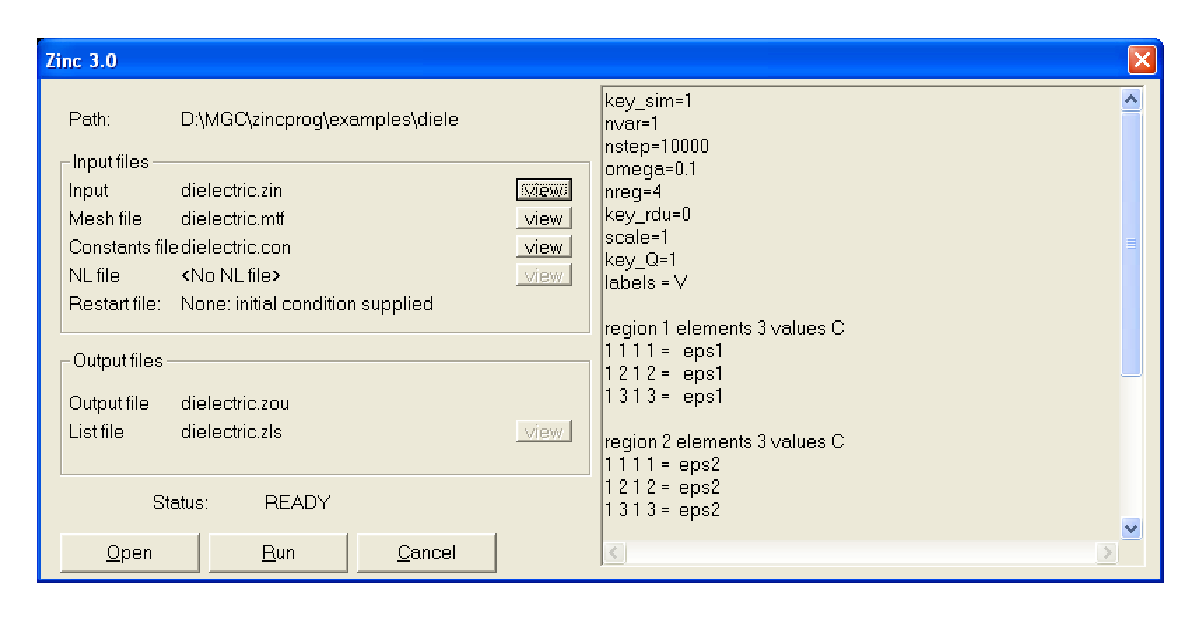
\includegraphics{zincpic}}
  \caption{Program \zinc}
  \label{zincpic}
\end{figure}

\section{Mesh definition file \var{file.mtf}}
\label{mtf}

The MTF file is normally generated by Zmesh (Chapter \ref{zmeshchap}), but you
can generate it manually if needed. The full specification of this
file is given in Appendix \ref{mtfdesc}.

\section{Material/physics file \var{file.zin}}
\label{zincini}
The file consists of several parts, which may be given in any order:
\begin{enumerate}
\item Control variables of the form \var{variable=value}. This
  includes number of iteration steps to run, the simulation type etc.
\item Region specification blocks. Associates material properties and
  physics with each region number. These blocks start with \var{region
    xx elements...} or \var{region xx nodes...}, see below.
\item Surface statements applying Neuman boundary conditions (begin
  with the \var{surface} command.)
\item The initial condition (\var{init}). This is followed by
  \var{nvar} lines of specifying the initial state of each simulation
  variable.
\end{enumerate}

In the ZIN file, horizontal line spacing is
unimportant and comment lines may be inserted beginning with
\var{!}. Lines may be continued using the ampersand (\&)
character, for example:
\begin{verbatim}
  solver= &
GMRES_DIAG    ! Great solver...
\end{verbatim}
is the same as
\begin{verbatim}
  solver=GMRES_DIAG
\end{verbatim}

\subsection{Control variables}
\label{zinctrl}

First of all, some background is needed on how to solve FE
systems. Considering first static problems, \zinc\ converts the PDEs
specified by the user in Chapter 4 into a set simultaneous linear
equations. In linear problems, these equations only need to be solved
once. \zinc\ will use the solver given as \var{solver} below and
iterate a maximum of \var{itmax} times or until a convergence of
\var{tol} is achieved (whichever happens first). For non-linear
problems, \zinc\ needs to solve sets of linear equations \emph{\var{nstep}
times}, updating the matrices each time. Thus the user must also
specify \var{nstep} for non-linear problems.

\zinc\ has many iterative solvers as described below (eg GMRES, SOR) and one
\emph{direct solver} called UMFPACK. An iterative solver starts with
the initial guess provided by the user (specified in the \var{init}
block) and moves towards the solution by an iterative process. The
problem is that attaining the solution may take a long time and is
dependent on the quality of the initial guess. The benefit of
iterative solvers is they take less memory and so are particularly useful
for large problems.

Direct solvers, on the other hand, solve the linear equations directly
by Gaussian elimination, without refering to the initial state at
all. This is just how we might solve a linear equation like $2x+1=3$
with pen and paper: by direct algebraic manipulation with no need to
guess an initial value for $x$. Of course in FE there are many
thousands or even millions of simultaneous equations but the principle
is the same. Direct solvers are guaranteed to get the right answer but
take more memory. \zinc\ supports only the UMFPACK direct solver.

So far we have discussed how to solve a linear set of equations. For
linear problems that is all we need to do. For non-linear problems,
\zinc\ solves the non-linear equations by \emph{solving linear equation sets
multiple times} (in fact \var{nstep} times). There are two ways
\zinc\ can do this: using a simple iteration scheme and with the
Newton-Raphson method. For the latter, specify \var{Newton=YES} in the ZIN
file. The Newton method is more likely to converge on a solution but
the user must also provide derivatives of matrix quantities. So, if a C-matrix
element varies as $C=V^2+0.5(\d V/\d x)$, for example, the user must
also tell \zinc\ that $\d C/\d V = 2V$ and $\d C/\d V_x=0.5$ where
$V_x=\d V/\d x$. More details of how to do this is given in \sect{newtonspec}. For
now we note that \var{Newton=YES} is more complicated but could give
better results for highly non-linear problems.

Turning now to transient problems, the parameter \var{nstep} is just
equal to the number of timesteps to be computed. For non-linear transient
problems, \zinc\ updates the FE matrices every \var{nstrideNL} steps
to correspond to the way that material properties have changed. Only 1
solver is defined called \var{solver=TRANSIENT}.

The control variables are as follows:
\begin{description}
\item[nvar] Number of variables to solve for. Eg, 1 in electrostatics,
  4 in piezoelectrics etc.

%\item[ndim] Number of spatial dimensions to solve for: 1, 2 or 3 (default 3)

\item[nstep] For transient problems, this is the total number of time
  steps, so that the simulation covers a time period of
  \var{nstep*tstep}. For non-linear static problems, it is the number
  of matrix updates (non-linear problems are solved by repeatedly
  solving linear problems and updating material properties
  between. This process is repeated \var{nstep} times). Ignored for
  linear static problems.

\item[tstep] Time interval for transient problems. Total time
  simulated is \var{nstep*tstep}.

\item[solver] TRANSIENT: transient run. The remaining solvers are all
  static as follows: SOR: Static run with Successive Over Relaxation;
  SOR\_SYM: Symmetical successive over-relaxation; GMRES\_DIAG:
  General Minimal Residual Method solver (diagonally scaled);
  GMRES\_LU: GMRES solver (Incomplete LU factorisation); BCG\_DIAG:
  Biconjugate Gradient solver (Diagonally scaled); BCG\_LU:
  Biconjugate Gradient solver (Incomplete LU factorisation);
  CONJ\_DIAG: Conjugate Gradient method with diagonal scaling;
  CONJ\_CHOLESKY: Conjugate Gradient method with incomplete Cholesky
  factorisation. The last two should be used only for positive
  definite systems. Finally UMFPACK is a direct solver.

\item[omega] Successive over-relaxation parameter for
  \var{solver=SOR,SOR\_SYM}. This dimensionless parameter should be
  between 1-2 but you may consider a value less than 1 when
  convergence is difficult.

\item[tol] Tolerance for the convergence of linear equations. If \zinc\ estimates it
  has solved the equations to better than \var{tol} accuracy, it will
  end the simulation. Otherwise it will continue to a maximum of
  \var{itmax} iterations. Ignored if solver=TRANSIENT or UMFPACK. (default $10^{-6}$)

\item[itmax] This is the maximum number of iterations carried out by
  the solver. If \var{tol} accuracy is achieved, the simulation will
  terminate early. (default 1000)

\item[newton] Used only for non-linear static problems. If newton=YES,
  \zinc\ will iterate towards the solution using derivative
  information via the Newton-Raphson method (In this case, the user
  must supply additional callback functions, see \sect{newtonspec}). Otherwise, a
  simpler substitution method is used which does not use derivatives but is less
  likely to converge in very non-linear cases. (default=NO)

\item[removefixed] if YES, fixed (clamped) nodes are removed from the
  set of equations at the beginning leaving a smaller set of
  equations. This is generally a good idea but it is not currently
  supported for NEWTON iteration schemes. (default=YES)

\item[restart] Specify a restart file which must be a valid
  \zinc\ .ZOU file from a previous run. Eg
  \var{restart=dielectric.zou}. The \var{init} section \sect{initsec}
  defines how the data in the restart file is to be used. (If the
  previous simulation was transient, \var{filename.zou} will consist
  of several snapshots. In this case \zinc\ automatically reads the
  last one of these from the specified restart file and continues from
  that). If \var{restart} is not specified, no restart will occur.

\item[scale] factor to multiply distances found in \var{zinc.mtf} to
  put them in metres (or whatever distance unit in implied in the PDEs
  that have been set). E.g. if the dimensions in the \var{zinc.mtf}
  file are mm and natural units are metres, set scale to
  0.001. (Default 1).

\item[nstride] Convergence information is written every nstride
  iteration steps. In transient problems, snapshots of the solution
  are also written every nstride steps. (default 10)

\item[nstrideNL] Used for non-linear transient problems only. This is
  the frequency to update matrices. They are updated every nstrideNL
  steps based on the current solution.

\item[export] NONE: No export. PARAVIEW: Export to Paraview format
  \var{.vtk} files. (default NONE)

\item[labels] List of \var{nvar} labels for the variables being
  simulated. E.g., in a thermo-electric simulation, we might have
  \var{labels T V}. If no labels command is used, variable names
  default to \var{u1}, \var{u2} etc

\item[zou\_format] Controls the format of the output file
  \var{file.zou}. BINARY: export in binary format (recommended);
  ASCII: export in ASCII format text file. (default: BINARY).

\item[rst\_format] Controls the format of the restart file
  specified using \var{restart} (see above). BINARY: restart file is in binary format;
  ASCII: restart file is in ASCII format. (default: BINARY).

\item[residual] (advanced) Optionally displays a residual of the
  solution. NONE: No residual plot. PIVOTS or UNKNOWNS: output
  residual map in \emph{additional file} \var{filename.resid}. This
  can be read into \var{Zmesh} showing graphically how well equations
  have been solved at each point. You can examine the left hand side
  (LHS) and right hand side (RHS) or each equation and the difference
  between them (residual) which should be close to zero. PIVOTS means
  that pivot (lead diagonal) values are gathered into the LHS (and
  everything else on the RHS) while UNKNOWNS means all unknown values
  are on the LHS and fixed values (deriving from Dirichlet boundaries
  and source terms) are on the RHS (default: NONE)
\end{description}

\subsection{Region specification blocks}
\label{regionspec}

These have the form
\begin{verbatim}
region i [keyword] [matrix name]  
:
end
\end{verbatim}
If keyword is ``elements'' the block specifies material properties of
elements with region number \texttt{i}. The matrix name must be
\texttt{C, a} or \texttt{f}. If keyword is ``nodes'' the block specifies
nodes which are fixed (Dirichlet boundary conditions) and ``matrix
name'' is not used. Within the region block we have entries of the form
\begin{verbatim}
<list of indices> = value
\end{verbatim}
The number of indices is: 4 for C-matrix, 2 for a-matrix and 1 for f-matrix. Eg
\begin{verbatim}
region 2 elements a
  1 1 = 1.0
  2 2 = 2.0
\end{verbatim}
would specify $a_{1,1}=1$ and $a_{1,2}=2$ in the \zinc\ a-matrix for region 2.
Additionally, for specifying the C-matrix only, it is possible to enter an
entire $3\times3$ submatrix in one go. This is in the form
\begin{verbatim}
region 1 elements C
  i j = [v1, v2, v3, v4, .... v9]
:
end
\end{verbatim}
where i,j specify the submatrix number. For example to enter the matrix
\begin{equation}
  C=
  \left(\begin{array}{ccc|ccc}
    \sigma_{11} & 0 & 0 & 0 & 0 & 0\\
    0 & \sigma_{22} & 0 & 0 & 0 & 0\\
    0 & 0 & \sigma_{33} & 0 & 0 & 0\\ \hline
    0 & 0 & 0 & k & 0 & 0\\
    0 & 0 & 0 & 0 & k & 0\\
    0 & 0 & 0 & 0 & 0 & k
  \end{array}\right)
\end{equation}
for region 1, we would use
\begin{verbatim}
region 1 elements C
   1 1 = [sig11, 0, 0, &
          0, sig22, 0, &
          0, 0, sig33]

   2 2 = [k, 0, 0, &
          0, k, 0, &
          0, 0, k]
end
\end{verbatim}
Recall that \verb+&+ is the continuation character. We could equally have entered
\begin{verbatim}
region 1 elements C
   1 1 = [sig11, 0, 0, 0, sig22, 0, 0, 0, sig33]
   2 2 = [k, 0, 0, 0, k, 0, 0, 0, k]
end
\end{verbatim}
but this is not so readable. We can, of course enter, C-matrix elements individually as, for example,
\begin{verbatim}
region 1 elements C
    2    2    1    2 = sig11
:
end
\end{verbatim}
which specifies $C_{2212}=$\var{sig11}. In this case, the \emph{first and
third} components (2,1) specify the submatrix index and the \emph{second and
fourth} (2,2) are the position within that matrix. Generally it is clearer to
specify submatrices \verb+[1,2,3...,9]+ when specifying the C-matrix rather than
individual elements.

Note that expressions may be entered in place of literal constants, a
facility which allows spatial variation of material properties and/or
non-linearity. See \sect{expressions}.

An alternative, if \var{labels} has been specified, is to enter the
variable names and the directions \var{x,y,z} instead of index numbers. Thus we might have
\begin{verbatim}
region 1 elements C
  V x V x = 0.31100E+11
end
\end{verbatim}
which means the same as
\begin{verbatim}
region 1 elements C
  1 1 1 1 = 0.31100E+11
end
\end{verbatim}
Both commands set $C_{1111}=0.31100\times10^{11}$ but the former may be
more helpful as it gives a clearer idea what the meaning of this C
element is.

Coefficient $a$ has 2 components so an entry in the list might be
\begin{verbatim}
  1 1 = -3.03983816e15 OR
  V V = -3.03983816e15
\end{verbatim}
which specifies $a_{11}=-3.03983816\times10^{15}$ (SI units). Coefficient
f has 1 component so an entry might be
\begin{verbatim}
  1 = 0.5 OR
  V = 0.5
\end{verbatim}
which specifies $f_1=0.5$ (SI units)

\textbf{Note:} Zero values need not be entered, these are assumed by
default. The full specification of \caf\ will be written in
\var{filename.zls}, it is advisable to check this.

If the keyword is ``nodes'' then we specify nodes to have fixed values of
one or more variables. There then follows a list of fixed variables of form
variable number (or symbol) = value. Eg, to fix variables 4 and 5 in
region 9 use: 
\begin{verbatim}
region 9 nodes
  4 = 0.04 
  5 = 0 
end
\end{verbatim}
or, if \var{labels} has been set
\begin{verbatim}
region 9 nodes
  T = 0.04 
  V = 0 
end
\end{verbatim}
(for example). The latter form is easier to read.

This fixes, $u_4=T=0.04$ and $u_5=V=0$ for all region 9 nodes. Variables
not specified default to \emph{not} being fixed. The specification of
all nodes and whether they are fixed is written out
\var{filename.zls}.

\subsection{Initial state specification}
\label{initsec}
It is also necessary to specify the initial state of the system. For
example, in a thermo-electric problem, with \var{labels} \var {T, V}
we could have
\begin{verbatim}
  init
     T=1
     V=0
  end
\end{verbatim}
which sets the initial temperature to 1 and the initial voltage to
zero throughout the simulation. Initialisations can use  expressions in terms of
(x,y,z) and/or parameters in the constants file, \var{.con} file, \sect{constfile}. (note that nonlinear
expressions like $V=T^2$ are not permitted). It is also possible
to set the initial state from a previous \zinc\ run. First, nominate
the file to continue from using \var{restart}, \sect{zinctrl}. Then use the
\var{init} block to specify how variables will be initialised from the
content of the restart file using a variable name ``R''+ index
number. For example, considering again the thermo-electric problem,
\begin{verbatim}
  init
     T=1+x/2
     V=R4*2
  end
\end{verbatim}
This says that temperature should be initialised using the expression
$1+x/2$ (see \sect{expressions} for use of expressions) while the
voltage should be initialised from the 4th variable in the restart
file, multiplied by 2. E.g. if the previous run had variables, say,
\var{ux, uy, uz, V}, then \var{R4} is the voltage, V.

If you want very fine control over how the simulation starts, you
could write a program to generate the restart ZOU file directly from
the description given in Appendix \ref{zousec}.

\subsection{Initialisation override in region specification blocks}
The ``init'' block specifies global initialisation, but this can be
overridden on a per-region basis within region specification blocks, eg,
\begin{verbatim}
region 1 nodes
  init vEle=vCellAno
  wO=0
  wH2OCat=0
  cH3O=0
  cH2O=0
  vMem=0
end
\end{verbatim}
Here, \var{wO} etc are being clamped at zero but \var{vEle} is
\emph{initialised} to \var{vCellAno} (a parameter in the constants
file). This overrides the initialization specification in the global
\var{init} block. The semantics for initialisation override are just
the same as a regular node region blocks but with the token ``init''
preceding the statement.

\subsection{Specifying Neumann boundaries at surfaces}
\label{neumanspec}

So far we have set material properties/physics within
regions and Dirichlet boundaries on nodes. The other boundary
condition is Neumann boundary which has the general form
\begin{equation}
  n_jC_{ijkl}u_{k,l}+q_{ik}u_k=g_i
\end{equation}
The $q$ and $g$ values default to zero. To set them non-zero, we
identify a surface between to volumetric regions (see \f{outer}) and attach
parameters using the command
\begin{verbatim}
surface i-j [matrix name]
:
end
\end{verbatim}
where $i$ and $j$ are the two regions, $N$ is the number of entries to
follow and ``matrix name'' must be ``g'' or ``g''. A typical example is
\begin{verbatim}
surface 1-2 g
   1 = 1.0
   2 = 2.0
   3 = 3.0
end
\end{verbatim}
If labels have been defined, these can be used in place of indices. Eg in an
electrostatic problem with labels (displacements) \var{u, v, w}
\begin{verbatim}
surface 1-2 g
   u = 1.0
   v = 2.0
   w = 3.0
end
\end{verbatim}
As shown in \f{outer}, the simulation is conceptually surrounded by
regions called XMAX etc. Thus, 1-XMAX is the surface between region 1
and the maximum-x edge of the simulation. To specify g on this surface use
\begin{verbatim}
surface 1-XMAX g
   u = 1.0
   v = 2.0
   w = 3.0
end
\end{verbatim}

\section{Expressions}
\label{expressions}

\begin{table}
  \begin{tabular}{l|l}
    Name & Meaning \\ \hline
    pi & The constant $\pi$\\
    i & The constant $\sqrt{-1}$\\
    x & x position in space\\
    y & y position in space\\
    z & z position in space\\
    nx & x-component of unit normal (used for \qg\ only)\\
    ny & y-component of unit normal (used for \qg\ only)\\
    nz & z-component of unit normal (used for \qg\ only)\\
    u1 & first variable value\\
    u2 & second variable value\\
    :  & :\\
    u1x & derivative of first variable with respect to x\\
    u1y & derivative of first variable with respect to y\\
    u1z & derivative of first variable with respect to z\\
    u2x & derivative of second variable with respect to x\\
    u2y & derivative of second variable with respect to y\\
    u2z & derivative of second variable with respect to z\\
    : & :
  \end{tabular}
  \caption{Built-in variables which can be used in
    \zinc\ expressions. If the user defines the names of variables,
    these will be used in place of \var{u1, u2, u1x} etc (eg \var{V, T,
    Vx...} if labels are ``V'' and ``T''). The user may also reference
    constants in the \var{.con} file.}
  \label{vartab}
\end{table}

Instead of entering a literal constant like \var{1.0}, it is possible,
in \caf, \qg, nodal and initial specifications, to enter mathematical
expressions. The expression may depend on: the constants in
\var{filename.con}; the built-in variables \var{pi=3.14159,
  i=sqrt(-1)}; spatial variables \var{x,y,z}; and variables
corresponding to the dependent variables to be solved for. These last
are called \var{u1,u2,...u(nvar)}. Their derivatives are also
available and are called \var{u1x,u1y,u1z, u2x,u2y,u2z...}. However,
if \var{labels} has been set, these names are used instead. Thus, in a
thermo-electric system, with variables \var{T,V}, the standard
variables are \var{T, V, Tx, Ty, Tz, Vx, Vy, Vz}. The full set of
built-in variables in shown in \tab{vartab}.

Built-in variables \var{x,y,z} are the spatial coordinate in the
coordinate system specified in \var{filename.mtf}. If expressions are
given in terms of dependent variables $u1$ etc or their derivatives,
the simulation automatically becomes \emph{non-linear}. The functions
\var{sin, cos, tan, sqrt, exp, log, ln, abs, ang, real, imag, conjg,
  complex} may be used. Note that \var{log} is $\log_{10}$ while
\var{ln} is $\log_e$. Complex numbers may be constructed as
\var{a+b*i} or with the function \var{complex}:
\var{complex(a,b)}. Note that, although complex expressions are
allowed, all expressions must evaluate to real since \zinc\ operates
with real numbers only. If an expression is complex, it will be
truncated to real by discarding the imaginary part.

Examples of legal expressions include:
\begin{verbatim}
  1                                 ! same as 1.0, 1e0
  1+h/2                             ! h must be present in filename.con
  1e-6*(1+exp(-(x-x0)^2/(2*sig^2))) ! Gaussian, x0, sig must be in filename.con
  u1^2+u2y/u3z                      ! Depends on solution variables: non-linear
\end{verbatim}

Allowed operators include addition (+), multiplication (*), subtraction ($-$),
division (/), exponentiation (\verb+^+).

There are some restrictions on the size of expressions
\begin{enumerate}
\item The total string length of each expression is limited to 1000
  characters (including blank spaces)
\item The total number of ``items'' in each expression is limited to
  350. Here, an item is: a variable, a constant, an operator, an open
  or close bracket, a function like sin, cos, exp...
\item The maximum number of variables is 1000 (this includes constants
  in the \var{.con} file and those given in \tab{vartab}).
\end{enumerate}
In practice these restrictions still allow highly complex
equations. If your expressions are getting more complex than this, you
should consider using a DLL to specify the expression. See Section
\ref{nonlin}.

There are some restrictions on the type of expressions for each specification:
\begin{enumerate}
\item \qg\ specifications and node specifications (Dirichlet
  boundaries) may only be in terms of variables \emph{not} their
  derivatives. This is because derivative quantities are not
  defined on element boundaries or nodes.
\item Initialisation expressions may only be in terms of x,y,z and constants
\item \caf\ expressions may not use nx,ny,nz, these are reserved for \qg\ expressions
\end{enumerate}

\section{The constants file, \var{file.con}}
\label{constfile}

It is often convenient to define constants in the \var{file.con}
file. These can easily be changed between simulation without getting
into the details of the \var{file.zin} file (which also contains the
physics of the system). For instance, in an electrostatic simulation,
we might have the following \var{.con} file.
\begin{verbatim}
  eps0=8.854e-12
  eps1=eps0
  eps2=2*eps0
\end{verbatim}
thus setting up permittivities in various regions. In the \var{file.zin} file, we could then have
\begin{verbatim}
  region 1 elements C 
     1 1 1 1 = eps1
     1 2 1 2 = eps1
     1 3 1 3 = eps1
  end

  region 2 elements C 
     1 1 1 1 = eps2
     1 2 1 2 = eps2
     1 3 1 3 = eps2
  end
\end{verbatim}

The \var{.con} file contains a series of lines of the form
\begin{verbatim}
  var = value
\end{verbatim}
Constants may be defined \emph{in terms of pervious constants} but not
later ones. Thus the following \var{.con} file would be illegal
\begin{verbatim}
  eps1=eps0     ! eps0 not yet defined
  eps2=2*eps0
  eps0=8.854e-12
\end{verbatim}
The usual expression rules apply for expressions in the constants file.

\section{Advanced, non-linear simulations}
\label{nonlin}
For linear simulations, each of the numbers specifying \caf\, \qg\ is:
either a constant or evaluates to a constant OR depends only on
\var{x,y,z}. In non-linear simulations, one or more \caf\,
\qg\ numbers (or Dirichlet boundary values) depends on the solved-for
variables (\var{u1} etc) through an expression. As described in
\sect{expressions}, expressions can be entered directly, for example:
\var{1+sin(x/2)+stiffness*u1*u2x} etc. \zinc\ can parse such one-line formulas using an
internal parser.

These expressions allow simple non-linearity but there is a more
advanced technique when the \caf\, \qg\ expressions become
complicated, perhaps requiring an actual computer program to
generate. In this case the user should enter a \emph{token} beginning
with \verb+$+ instead of a number for the \caf\ and \qg\ values. For
example, a token might be \verb+$copper_stiffness+. This token is
passed through to functions \var{Cfun, afun, ffun, gfun, qfun, BCfun}
which the user must provide in \var{file.dll}. As the names suggest
\var{cfun} etc are used to set the \caf\ and \qg\ values while
\var{BCfun} is used for Dirichlet boundary conditions, i.e., for node
specification in ``\var{region x nodes ...}'' blocks.  An example of
\var{ffun} in Fortran would be
\begin{verbatim}
function ffun(label,x,y,z,ur,dur,nvar,istep, &
              ireg,iregup,rnode,vec,imax,jmax,kmax)

  implicit none
  character(*) label
  integer nvar,istep,imax,jmax,kmax
  double precision ffun,x,y,z,ur(nvar),dur(nvar,3)
  integer ireg(0:imax,0:jmax,0:kmax),iregup(0:imax,0:jmax,0:kmax)
  double precision rnode(0:imax,0:jmax,0:kmax,3),vec(*)


  if (label=='$ohmic_heating') then
      ffun=dur(1,1)**2+dur(1,2)**2+dur(1,3)**2

      ! other options...

  endif
  
end function ffun
\end{verbatim}
What's happening here, is that Zinc is asking for the value of the
\textbf{f} matrix element identified with the token
\verb+ohmic_heating+ in the \var{file.zin} input file. Zinc provides
the current position in space as \var{x,y,z} and also presents the
local solution as \var{ur(i)}$=u_i$ and its derivatives as
\var{dur(i,j)}$=\d u_i/\d x_j$. Some other parameters are provided
which are described in more detail below.

Note that the \emph{only} purpose of the function is to return a
single number (the function return value). The function should not
alter any of the input arguments. A large number of arguments are
passed for information, but user-written functions will likely make
use of only some of them. In the example given, only the argument
\var{dur} is being used: this provides the spatial derivative of the
solved-for variables in x, y and z.

In C, the function \var{ffun} would look like this
\begin{verbatim}
double ffun(char *label, double *x, double *y, double *z, 
            double ur[1], double dur[3][1], int *nvar, int *istep, 
            int *ireg, int* iregup, double *vec, 
            int *imax, int *jmax, int *kmax, int length)
{
  double Ex,Ey,Ez;

  if (equal(label,length,"$ohmic_heating")){
      Ex=dur[0][0];
      Ey=dur[1][0];
      Ez=dur[2][0];

      return Ex*Ex+Ey*Ey+Ez*Ez;
  }

  // other options...
  
}
\end{verbatim}
Note that the string passed (\var{label}) in is not null-terminated
but of fixed length \var{length} and is hence dealt with using our own
\var{equal} function as shown in \f{equal}. Also the C \var{dur}
matrix is transposed compared to the matrix in the Fortran example
since the two languages arrange multi-dimensional arrays
differently. Chapter 3 of the Tutorial Manual shows a fuel cell
simulation using Fortran and C non-linear functions using the free gcc
compiler. You should try compiling and running this example before
preparing your own advanced non-linear simulations.

\begin{figure}
\begin{verbatim}
  
int equal(char *s, int length, char *t)
{

  int i,len1,len2;

  for (i=0;i<length;i++){
    if (s[i]==' ') break;
  }

  len1=i;

  for (i=0;i<length;i++){
    if (t[i]=='\0') break;
  }

  len2=i;

  if (len1==len2){
    for (i=0;i<len1;i++)
      if (s[i]!=t[i]) return 0;
      
    return 1;
  }
  else
    return 0;
}
\end{verbatim}
\caption{A simple function to compare strings \var{s} (fixed length
  \var{length}) and \var{t} (null terminated)}
\label{equal}  
\end{figure}

In the example just described, the program substitutes the value
\begin{equation}
  \left(\frac{\d u_1}{\d x_1}\right)^2+
\left(\frac{\d u_1}{\d x_2}\right)^2+
\left(\frac{\d u_1}{\d x_3}\right)^2
\end{equation}
wherever the token \verb+$ohmic_heating+ appears in
\var{filename.zin}. For example in an electrostatic run, $u_1=V$, the
electric potential so the above expression evaluates to $|E|^2$.  In
functions \var{cfun, afun, ffun, qfun, gfun}, \var{ur(i)}$=u_i$,
\var{dur(i,j)}$=\d u_i/\d x_j$.

The variables passed to the non-linear functions are as follows
\begin{description}
  \item[label] A string containing the token specified in the input
    file, including the initial \$ (not NULL-terminated).
  \item[x, y, z] The current spatial position (given by reference to the
    meshing (double precision\footnote{8 byte reals})
  \item[ur] Array of length \var{nvar} containing the current solution
    at (x,y,z), \var{ur(i)}$=u_i$ (double precision)
  \item[dur] Array of size \var{dur(nvar,3)} so that
    \var{dur(i,j)}$=\d u_i/\d x_j$ at (x,y,z) (double precision)
  \item[nvar] Number of variables (integer)
  \item[istep] The current iteration step. In transient problems the
    current time is \var{istep*tstep} where \var{tstep} is described
    in \sect{zinctrl}. \var{istep} may be useful in static problems as
    well since the non-linear routines can use it to find out when the
    \zinc\ matrices have been updated.
  \item[nx, ny, nz] (only available when forming $\vec q$ and $\vec g$
    matrices.) The current outward surface unit normal pointing \emph{from}
    the first specified region \emph{to} the second. eg for a surface
    beginning \var{surface 1-2 3 values g}, the normal provided would
    be \emph{from} region 1 \emph{to} region 2.  (double precision)
  \item[imax, jmax, kmax] The number of elements in each direction. (see
    Appendix \ref{mtfdesc})
  \item[ireg, iregup, rnode, vec] These multi-dimensional arrays
    provide full information about meshing and the current solution at
    every node (not just the local point: x,y,z). These parameters are for advanced users and are
    described in detail in Appendix \ref{mtfdesc}
\end{description}

The full template the for the non-linear functions in \var{file.dll}
is shown in \f{template} and \f{template2}. The function \var{scanfun}
is used by \zpp, which is described in \chap{zppchap}. The full
template for C-language non-linear functions is given in
\f{ctemplate}.

Note that derivative quantities are available for forming
\caf\ matrices but not for \qg\ matrices (since derivatives are not
defined on element boundaries). On the other hand, only \var{qfun,
  gfun} have access to the local surface normal since (nx,ny,nz) this
concept is only meaningful on a surface.

\begin{figure}
\begin{verbatim}

function cfun(label,x,y,z,ur,dur,nvar,istep, &
          ireg,iregup,rnode,vec,imax,jmax,kmax)
   character(*) label
   integer nvar,istep,imax,jmax,kmax
   double precision cfun,x,y,z,ur(nvar),dur(nvar,3)
   integer ireg(0:imax,0:jmax,0:kmax),iregup(0:imax,0:jmax,0:kmax)
   double precision rnode(0:imax,0:jmax,0:kmax,3),vec(*)
end function cfun
     
function afun(label,x,y,z,ur,dur,nvar,istep, &
          ireg,iregup,rnode,vec,imax,jmax,kmax)
   character(*) label
   integer nvar,istep,imax,jmax,kmax
   double precision afun,x,y,z,ur(nvar),dur(nvar,3)
   integer ireg(0:imax,0:jmax,0:kmax),iregup(0:imax,0:jmax,0:kmax)
   double precision rnode(0:imax,0:jmax,0:kmax,3),vec(*)
end function afun

function ffun(label,x,y,z,ur,dur,nvar,istep, &
          ireg,iregup,rnode,vec,imax,jmax,kmax)
   character(*) label  
   integer nvar,istep,imax,jmax,kmax
   double precision x,y,z,ffun,ur(nvar),dur(nvar,3)
   integer ireg(0:imax,0:jmax,0:kmax),iregup(0:imax,0:jmax,0:kmax)
   double precision rnode(0:imax,0:jmax,0:kmax,3),vec(*)
end function ffun

\end{verbatim}
\caption{Template for Fortran non-linear functions,
  \var{file.dll}. Note that the arguments on the second line of each
  function declaration are regarded as ``advanced'' and may be ignored
  by most users. This template is supplied as \var{nltemplate.f90} in
  the Zinc install directory (continued in next figure)}
\label{template}
\end{figure}

\begin{figure}
\begin{verbatim}
     
function qfun(label,x,y,z,nx,ny,nz,ur,nvar,istep, &
          ireg,iregup,rnode,vec,imax,jmax,kmax)
   character(*) label
   double precision qfun,x,y,z,nx,ny,nz,ur(nvar)
   integer nvar,istep,imax,jmax,kmax
   integer ireg(0:imax,0:jmax,0:kmax),iregup(0:imax,0:jmax,0:kmax)
   double precision rnode(0:imax,0:jmax,0:kmax,3),vec(*)
end function qfun
     
function gfun(label,x,y,z,nx,ny,nz,ur,nvar,istep, &
          ireg,iregup,rnode,vec,imax,jmax,kmax)
   character(*) label
   double precision gfun,x,y,z,nx,ny,nz,ur(nvar)
   integer nvar,istep,imax,jmax,kmax
   integer ireg(0:imax,0:jmax,0:kmax),iregup(0:imax,0:jmax,0:kmax)
   double precision rnode(0:imax,0:jmax,0:kmax,3),vec(*)
end function gfun

function BCfun(label,x,y,z,ur,nvar,istep, &
          ireg,iregup,rnode,vec,imax,jmax,kmax)
   character(*) label
   double precision BCfun,x,y,z,ur(nvar)
   integer nvar,istep,imax,jmax,kmax
   integer ireg(0:imax,0:jmax,0:kmax),iregup(0:imax,0:jmax,0:kmax)
   double precision rnode(0:imax,0:jmax,0:kmax,3),vec(*)
end function BCfun

function scanfun(label,x,y,z,nx,ny,nz,ur,dur,nvar)
  character(*) label
  integer nvar
  double precision scanfun,x,y,z,nx,ny,nz,ur(nvar),dur(nvar,3)
end function scanfun

\end{verbatim}
\caption{(Continued from previous figure)}
\label{template2}
\end{figure}

\begin{figure}
\begin{verbatim}
double cfun(char *label, double *x, double *y, double *z, 
       double ur[1], double dur[3][1], int *nvar, int *istep, 
       int *ireg, int *iregup, double *rnode, double *vec, 
       int *imax, int *jmax, int *kmax, int length) ;

double afun(char *label, double *x, double *y, double *z, 
       double ur[1], double dur[3][1], int *nvar, int *istep, 
       int *ireg, int *iregup, double *rnode, double *vec, 
       int *imax, int *jmax, int *kmax, int length) ;

double ffun(char *label, double *x, double *y, double *z, 
       double ur[1], double dur[3][1], int *nvar, int *istep, 
       int *ireg, int *iregup, double *rnode, double *vec, 
       int *imax, int *jmax, int *kmax, int length) ;

double qfun(char *label, double  *x, double  *y, double  *z, 
                         double *nx, double *ny, double *nz,
       double ur[1], int *nvar, int *istep, 
       int *ireg, int *iregup, double *rnode, double *vec, 
       int *imax, int *jmax, int *kmax, int length) ;

double gfun(char *label, double  *x, double  *y, double  *z, 
                         double *nx, double *ny, double *nz,
       double ur[1], int *nvar, int *istep, 
       int *ireg, int *iregup, double *rnode, double *vec, 
       int *imax, int *jmax, int *kmax, int length) ;

double BCfun(char *label, double *x, double *y, double *z,
       double ur[1], int *nvar, int *istep, 
       int *ireg, int *iregup, double *rnode, double *vec, 
       int *imax, int *jmax, int *kmax, int length) ;

double scanfun(char *label, double  *x, double  *y, double  *z,
                            double *nx, double *ny, double *nz,
       double ur[1], int *nvar, int length) ;

\end{verbatim}
\caption{Template for C non-linear functions, \var{file.dll}. Here we
  have assumed that there is 1 variable. The C functions receive an
  additional variable, \var{length}, which is the length of the string
  \var{label}. This string is \emph{not} null terminated. User-written
  functions should not alter parameters passed in. This template is
  provided in \var{nltemplate.c}}
\label{ctemplate}
\end{figure}

\section{Non-linear problems using the Newton-Raphson method (advanced)}
\label{newtonspec}

To solve problems of this kind (with NEWTON=YES) we need to specify, not only the
values of \caf\ and \qg\ but also their derivatives. This is needed so that
\zinc\ can form the Jacobian matrix. To return to our example with
Ohmic heating we would use
\begin{verbatim}
ohm.zin:

region 3 elements f
  1 = $ohmic_heating
end
\end{verbatim}
with the \var{ohm.dll} file given in \f{newtonex}.
\begin{figure}
\begin{scriptsize}
\begin{verbatim}
function ffun(label,x,y,z,ur,dur,nvar,istep, &
              ireg,iregup,rnode,vec,imax,jmax,kmax)

  implicit none
  character(*) label
  integer nvar,istep,imax,jmax,kmax
  double precision ffun,x,y,z,ur(nvar),dur(nvar,3)
  integer ireg(0:imax,0:jmax,0:kmax),iregup(0:imax,0:jmax,0:kmax)
  double precision rnode(0:imax,0:jmax,0:kmax,3),vec(*)


  if (label=='$ohmic_heating') then
      ffun=dur(1,1)**2+dur(1,2)**2+dur(1,3)**2

      ! other options...

  endif
end function ffun

subroutine dffun_du(label,x,y,z,ur,dur,nvar,istep, &
                    ireg,iregup,rnode,vec,imax,jmax,kmax,dfdu)
  implicit none
  character(*) label
  double precision dfdu(nvar),x,y,z,ur(nvar),dur(nvar,3)
  integer nvar,istep,imax,jmax,kmax
  integer ireg(0:imax,0:jmax,0:kmax),iregup(0:imax,0:jmax,0:kmax)
  double precision rnode(0:imax,0:jmax,0:kmax,*),vec(*)


  if (label=='$ohmic_heating') then
      dfdu(1)=0
  else if (...)

      ! other options...

  endif
  
end subroutine dffun_du

subroutine dffun_ddu(token,x,y,z,ur,dur,nvar,istep, &
                     ireg,iregup,rnode,vec,imax,jmax,kmax,dfddu)
  implicit none
  character(*) token
  integer nvar,istep,imax,jmax,kmax
  double precision dfddu(nvar,3),x,y,z,ur(nvar),dur(nvar,3)
  integer ireg(0:imax,0:jmax,0:kmax),iregup(0:imax,0:jmax,0:kmax)
  double precision rnode(0:imax,0:jmax,0:kmax,*),vec(*)

  if (label=='$ohmic_heating') then
      dfddu(1,1)=2*dur(1,1)
      dfddu(1,2)=2*dur(1,2)
      dfddu(1,3)=2*dur(1,3)
  else if (...)

      ! other options...

  endif
end subroutine dffun_ddu
\end{verbatim}
\end{scriptsize}
\caption{Example callback functions for Newton-Raphson method (file \var{ohm.f90 -> ohm.dll})}
\label{newtonex}
\end{figure}
so we are saying
\begin{eqnarray}
  f=(\d V/\d x)^2+(\d V/\d y)^2+(\d V/\d z)^2\\
  \var{dfdu(1)}=\d f/\d V = 0\\
  \var{dfddu(1,1)}\equiv \d f/\d V_x=\var{2*dur(1,1)}\equiv 2(\d V/\d x)\\
  \var{dfddu(1,2)}\equiv \d f/\d V_y=\var{2*dur(1,2)}\equiv 2(\d V/\d y)\\
  \var{dfddu(1,3)}\equiv \d f/\d V_z=\var{2*dur(1,3)}\equiv 2(\d V/\d z)
\end{eqnarray}
The return values of \var{dffun\_du} and \var{dffun\_ddu} are given by matrices,
\begin{eqnarray}
  \var{dfdu(i)}=\frac{\d f}{d u_i}\\
  \var{dfddu(i,j)}=\frac{d f}{\d(\d u_i/\d x_j)}
\end{eqnarray}
The names of the derivative subroutines (void functions in C) follow
the function names for the matrix-specification functions themselves:
\begin{verbatim}
cfun ->  dcfun_du, dcfun_ddu
afun ->  dafun_du, dafun_ddu
ffun ->  dffun_du, dffun_ddu
\end{verbatim}
Currently the Newton-Raphson method is only supported for the C- and
f-matrices. If the other matrices contain non-linear terms, the
Newton-Raphson method cannot be used (it's OK for the other matrices
to be non-zero and linear). Furthermore, the Newton-Raphson method
only allows non-lineariy to be specified in callback functions (in a
DLL) using token replacement as shown in \eq{newtonex}. Single line
expressions are not supported eg
\begin{verbatim}
region 3 elements f
  1 = Vx^2+Vy^2+Vz^2   ! no good for Newton=YES
end
\end{verbatim}
works fine for ``standard'' non-linear calculations (newton=NO) but
not for the Newton-Raphson method. Finally, removeFixed is ignored for
Newton-Raphson calculations. If you break any of these restrictions,
\zinc\ will let you know and will not start the simulation.

In practice calculating the derivatives analytically is often tedious
so the user might want to approximate the derivatives in terms of the
function itself. See the fuel cell tutorial in the Tutorial Manual for
an example of how to do this.

\section{Examples of \zinc\ input files}

Refering to the simple ``sphere in a cube'' geometry shown in \f{coat},
\f{simpleex} shows a simple linear system to solve an electrostatic
problem with 1 V applied across the system. The inner sphere has
rel. permittivity 2 and the outer area rel. permittivity 1. The
initial voltage is 0 V.

In the second example, \f{nlex}, the permittivity depends on the
electric field as $(1+E/|E0|)*\epsilon$. In this example, we have
chosen a better guess for the initial voltage: a linear variation
between 0 (at $z=-h/2$, say) and 1 V (at $z=h/2$) on the top and
bottom plates. 

In the third example, \f{nlf90ex}, the exact same simulation is
carried out using non-linear functions in \var{dielectric.dll}. In
this case, \zinc\ will detect the presence of \var{dielectric.dll} and
link it to the \zinc\ core. 

\begin{figure}
\begin{verbatim}

dielectric.con:
===============
  eps0=8.854e-12


dielectric.zin
==============
  nvar = 1
  labels = V
  <other global commands>
  :

  region 1 elements 3 values C
    V x V x = eps0
    V y V y = eps0
    V z V z = eps0

  region 2 elements 3 values C
    V x V x = 2*eps0
    V y V y = 2*eps0
    V z V z = 2*eps0

  region 3 nodes 1 value
    V = 1

  region 4 nodes 1 value
    V = 0

  init
    V=0
\end{verbatim}
  \caption{Simple linear electrostatic simulation, cf \f{coat}}
  \label{simpleex}  
\end{figure}

\begin{figure}
\begin{verbatim}
dielectric.con:
===============
  eps0=8.854e-12
  eps1=eps0
  eps2=2*eps0
  E01=1000   ! V/m
  E02=2000   ! V/m
  h=1e-3     ! m

dielectric.zin
==============
  nvar = 1
  labels = V
  <other global commands>
  :

  region 1 elements 3 values C
    V x V x = (1+sqrt(Vx^2+Vy^2+Vz^2)/E01)*eps1
    V y V y = (1+sqrt(Vx^2+Vy^2+Vz^2)/E01)*eps1
    V z V z = (1+sqrt(Vx^2+Vy^2+Vz^2)/E01)*eps1

  region 2 elements 3 values C
    V x V x = (1+sqrt(Vx^2+Vy^2+Vz^2)/E02)*eps2
    V y V y = (1+sqrt(Vx^2+Vy^2+Vz^2)/E02)*eps2
    V z V z = (1+sqrt(Vx^2+Vy^2+Vz^2)/E02)*eps2

  region 3 nodes 1 value
    V = 1

  region 4 nodes 1 value
    V = 0

  init
    V=0.5*(z/h+1)
\end{verbatim}
  \caption{Non-linear dielectric simulation}
  \label{nlex}  
\end{figure}

\begin{figure}

\begin{scriptsize}
\begin{verbatim}
dielectric.con:
===============
  h=1e-3    ! m

dielectric.zin
==============
  nvar = 1
  labels = V
  <other global commands>
  :

  region 1 elements 3 values C
    V x V x = $epsilon1
    V y V y = $epsilon1
    V z V z = $epsilon1

  region 2 elements 3 values C
    V x V x = $epsilon2
    V y V y = $epsilon2
    V z V z = $epsilon2

  region 3 nodes 1 value
    V = 1

  region 4 nodes 1 value
    V = 0

  init
    V=0.5*(z/h+1)

dielectric.dll (compiled from dielectric.f90)
=============================================

  function Cfun(label,x,y,z,ur,dur,nvar,istep, &
          ireg,iregup,rnode,vec,imax,jmax,kmax)
         
    character(*) label
    double precision Cfun,x,y,z,ur(nvar),dur(nvar,3)
    integer nvar,istep,imax,jmax,kmax
    integer ireg(0:imax,0:jmax,0:kmax),iregup(0:imax,0:jmax,0:kmax)
    double precision rnode(0:imax,0:jmax,0:kmax,3),vec(*)

    double precision, parameter :: eps0=8.854e-12
    double precision, parameter :: eps1=eps0,eps2=eps0*2
    double precision, parameter :: E10=1000, E20=2000
    double precision E

    E=sqrt(dur(1,1)**2+dur(1,2)**2+dur(1,3)**2)

    if (label=='$epsilon1') then
       Cfun=(1+E/E10)*eps1
    else if (label=='$epsilon2') then
       Cfun=(1+E/E20)*eps2
    endif
  end function Cfun

\end{verbatim}
\end{scriptsize}
  \caption{Non-linear dielectric simulation using DLL linkage}
  \label{nlf90ex}  
\end{figure}

\section{Zinc output files}

The following files are output by \zinc:

\begin{description}
  \item[filename.zls] Describes specification of run including \caf\,
    \qg\ values for each region and which nodes are fixed. Also shows
    initial and final distribution of energy in different regions.

  \item[filename.zou] The solution. Value of each variable at each node. This can be
    read by \zpp\ in post processing. The format is I, J ,K, variable
    number and value. 

  \item[filename.resid] (optional) Map of residuals showing how well each
    equation has been solved in solution obtained by \zinc. Can be
    read by \var{Zmesh}.

  \item[filenamexx.vtk] (optional) Snapshots in Paraview format. These are
    output every \var{nstride} timesteps if \var{export=YES}. In
    static runs, only one \var{.vtk} file is output at the end of
    the simulation.
\end{description}

\chapter{Zpp: the Zinc post processor}
\label{zppchap}

\begin{figure}
  \scalebox{0.8}{\includegraphics{zpppic}}
  \caption{Program \zpp, top, and automatically generated graph, bottom.}
  \label{zpppic}
\end{figure}

The \zinc\ Post Processor, \zpp, is shown in \f{zpppic}. Use ``Open''
to select a \var{file.zpp} input file (see below), then ``Run'' to
perform the post processing. The lower list box shows the output files
generated. Clicking on one and selecting ``graph'' shows a graph of
the line or plane scan selected (this button is deactivated for
integrals since these do not generate a graph). Again, individual
files can be examined using the ``view'' buttons.

\zpp\ allows complex views to be taken through the data and can also
perform integrations. You can plot the raw solved-for variables, their
derivatives or any function of these according to the usual rules for
expressions, \sect{expressions}. However, there is a new conditional
expression type, described in \sect{scanexpr}.  If you want to plot an additional
view, just add it to the input file and re-run \zpp. There is no need to re-run
\zinc\ itself just to get a different line scan! A basic view of the
simulation output can also be obtained using \zmesh, \sect{zmeshsec}.

\section{Zpp input files}
\label{zppinput}

\zpp\ reads \var{filename.zin, filename.mtf, filename.con} just as
\zinc\ does. It also reads its own file \var{filename.zpp} which has
the form
\begin{verbatim}
  <global commands>
  calculation 1
  calculation 2
  etc
\end{verbatim}

The global commands are

\begin{description}
\item[ftol] tolerance for finding points in elements. Must be less
then 1, typically order 1e-3. This is used when the program tries to
evaluate variable values at a point $(x,y,z)$ e.g. in line/plane
scans. If the point lies on the interface between elements there is
ambiguity and this tolerance is needed to find a value. (default 0.001)

\item[graph] NONE: do not create graphs; EPS: automatically create Encapsulated
  Postscript files (\var{*.eps}) using gnuplot (which must be
  installed); EMF: automatically create Enhanced Metafiles (\var{*.emf}) (default NONE)
\end{description}

Calculations have the form
\begin{verbatim}
  {calculation} [parameters] = expression
\end{verbatim}
The following calculations are supported
\begin{description}
  \item[linescan] Perform a linescan through the data. The parameters
    are \var{nline x1 y1 z1 x2 y2 z2} where \var{nline} is the number
    of points between coordinates (x1,y1,z1) and (x2,y2,z2)
  \item[planescan] Perform a planescan through the data. The
    parameters are \var{inorm pnorm a1 a2 b1 b2 Na Nb} where
    inorm=1,2,3 indicates a plane perpendiculer to x,y,z
    respectively. Within this plane (a1,b1) is the starting coordinate
    and (a2,b2) is the end coordinate. Na and Nb are the number of
    intervals along each direction. If inorm=1, a=y, b=z; if inorm=2,
    a=x, b=z; if inorm=3, a=x, b=y.
  \item[surfint] Integrate over a specified surface giving $\int
    (expression)\dee S$. The parameters are \var{ifrom ito} such that
    the surface exists between regions \var{ifrom} and \var{ito}. (the
    same concept as for Neuman boundaries, \sect{neumanbc}). The unit normal is
    available under variables \var{nx,ny,nz} and points from
    \var{ifrom} to \var{ito}. Derivative quantities may be used and
    are taken in the \var{ito} region evaluated on the surface.
  \item[volint] Integrate over a volume within the region specified
    giving $\int (expression)\dee V$. The single parameter is
    \var{region}, the region number to integrate over.
  \item[fdchk] Check solution is correct using finite difference
    check. \emph{This only works when all elements are cuboids
      parallel to coordinate axes}. Parameters are \var{norm plane
      equation}. For example \var{fdchk i 5 2} which means
    check equation 2 for plane $i=5$. For more details see Theory
    Manual, Section 8.
\end{description}

All calculations put their results into \var{.out} files named after
the simulation with a numerical subscript. Thus, \var{file01.out,
  file02.out} etc. Linescans and planescans produce data which can be
plotted in the form of a graph and indeed these graphs will be
generated, in the form of EPS of EMF picture files, if
\var{graph=EMF, EPS}. The integration commands simply output the
integral result in their output files and no picture is generated. The
interactive version of \zpp\ allows the user to view the graphs
generated immediately but in any case the graphs are written to the
simulation directory for the user to examine.

\section{Scan expressions}
\label{scanexpr}
Scan expressions basically have the same form as non-linear
expressions \sect{expressions}. Expressions can depend on solved-for
variables, the spatial position, the unit normal (surface intregration
only), and constants in the \var{.con} file, see \tab{vartab}.

However, it is also possible to use \emph{region dependent}
expressions of the form
\begin{verbatim}
  {reg1=expr1, reg2=expr2,...}
\end{verbatim}

Here, \var{reg1} etc is a valid region number, \var{expr1} is the
corresponding expression in the usual form \sect{expressions}. Note
that \emph{region expressions may not be nested}. Region expressions
are introduced because different regions have different material
properties and it is often necessary to chose the right one. An expression should be provided for each region traversed
during the scan, or an error will result. For example, to calculate
the x-component of the displacement field in the electrostatic calculation
shown in \f{simpleex}, we could use
\begin{verbatim}
  linescan [parameters] = -{1=eps1,2=eps2}*Vx
\end{verbatim}
In region 1, the expression evaluates to \var{-eps1*Vx}; in region 2,
it becomes \var{-eps2*Vx}.

\textbf{NOTE:} \zpp\ reads the files \var{filename.con, filename.zin}
so is aware of the constants specified e.g.,(\var{eps1,eps2}) and the
variable names, e.g., (\var{V}).

Alternatively, the user may refer to the function \var{scanfun} in
\var{filename.dll}. In this case, we use tokens beginning with \$, eg

\begin{verbatim}
  linescan [parameters] = $D

  :


  function scanfun(label,x,y,z,ur,dur,nvar)
    character(*) label
    integer nvar
    double precision scanfun,x,y,z,ur(nvar),dur(nvar,3)

    double precision, parameter :: eps0=8.854e-12
    double precision, parameter :: eps1=eps0,eps2=eps0*2
    double precision eps

    if (z.gt.0) then
      eps=eps1
    else
      eps=eps2
    endif

    scanfun=-eps*dur(1,1)
  end function scanfun
\end{verbatim}
would also generate the D-field. In this example, we assume that region 1 $z>0$
and region 2 $z<0$.

\section{Example calculations}

Let us assume an electrostatic calculation with $V$ as the only variable
(defined using the \var{labels} command in \var{.zin}). In that case
\begin{verbatim}
linescan 100    0.101 -0.3  -1.0     0.101 -0.3  +1.0 = V
\end{verbatim}
creates a line scan graph of voltage from (0.101,-0.3,-1.0) to (0.101,-0.3,+1.0)
with 100 points sampled.
\begin{verbatim}
linescan 100    0.101 -0.3  -1.0     0.101 -0.3  +1.0 = (V+1)^2/L
\end{verbatim}
creates the same graph but plotting $(V+1)^2/L$ assuming constant $L$ is defined in the \var{file.con} file.
\begin{verbatim}
linescan 100    0.101 -0.3  -1.0     0.101 -0.3  +1.0 = -Vz
\end{verbatim}
creates a plot of $-\d V/\d z$ which is the z component of electric
field (in this example).
\begin{verbatim}
  planescan      2  0.0   -1.0    1.0    -1.0    1.0    40  40 = &
-{1=eps1,2=eps2}*Vz
\end{verbatim}
creates a planescan in the plane $y=0.0$ with $x=[-1,1]$ and
$z=[-1,1]$. A $40\times40$ grid will be generated. The expression is
equal to \var{-eps1 Vz} in region 1 and \var{-eps2 Vz} in region
2. Recalling that $Vz$ is $\d V/d z$ and assuming the constants \var{eps1} and
\var{eps2} are the permittivities of regions 1 and 2, the expression
is the z component of electric displacement field (D-field).
\begin{verbatim}
  surfint 2 1 = eps0*(Vx*nx+Vy*ny+Vz*nz)
\end{verbatim}
Integrates over the surface between regions 1 and 2 and calculates
\begin{equation}
  \int \epsilon_0\vec E\cdot\vec n~\dee S
\end{equation}
In this case the electric field is evaluated on the region 1 side of
the interface (the second region specified) and the unit normal points
\emph{from} region 2 \emph{to} region 1. If region 1 is vacuum and
region 2 is a fixed potential electrode region, this integral will
give the electric charge on the electrode.

\section{Zpp output files}

\begin{description}
\item[filename01.out, filename02.out,..] Output files corresponding to
  the scans in \var{filename.zpp} in the order they were defined. In
  the transient case, all specified snapshots are output in each file,
  each separated by a double blank line. These files can be plotted
  with any graph plotter or spreadsheet. The timestep for each
  snapshot is indicaed in the file.

\item[filename01.eps, filename02.eps,..] In the case,
  \var{graph=EPS}, these are graphs are generated by gnuplot
  corresponding to the scans requested.

\item[filename01.emf, filename02.emf,..] In the case,
  \var{graph=EMF}, these are graphs are generated by gnuplot
  corresponding to the scans requested.
\end{description}

\begin{thebibliography}{9}
  \bibitem{gnuplot} Gnuplot graph plotter system. www.gnuplot.info
  \bibitem{wine} Wine. www.winehq.org
  \bibitem{crossover} CrossOver. www.codeweavers.com
  \bibitem{winebottler} WineBottler. winebottler.kronenberg.org
  \bibitem{fieldp} Field Precision Ltd, PO Box 13595, Albuquerque, New Mexico 87192 USA, www.fieldp.com
  \bibitem{meta} MetaMesh, Three-dimensional Conformal Mesh generator, Field Precision (2003).
\end{thebibliography}

\appendix

\chapter{Comsol's coefficient mode}
\label{comcoef}

Comsol allows the user to specify PDEs in the form
\begin{eqnarray}
  \div (-\vec C\grad \vec u -\vecc\alpha \vec u+\vecc\gamma)+\vec a\vec u+\vecc\beta\cdot\grad \vec u
=\vec f \label{comeq}\\
  \vec n\cdot(\vec C\grad\vec u+\vecc\alpha \vec u-\vecc\gamma)+\vec q\vec u=\vec g-\vec h^T\vecc\mu,
~~ \t{(Neumann)}\label{comneu}\\
  \vec h\vec u=\vec r,~~ \t{(Dirichlet)}
\end{eqnarray}
Here $\vec u=(u_1,u_2,...)$ where $u_1(x,y,z)$ etc are the independent
variables to be solved for. For example $u_1$ might be electrostatic
potential and $u_2$ temperature as in \sect{thermo}. One must set the
various components of $C$ etc so that, when \eq{comeq} is multiplied
out, we obtain the needed set of PDEs. Here, the meaning of grad and
div is non-standard. For example, with two variables, we define
\begin{eqnarray}
  \grad\vec u = (\grad u_1,\grad u_2)\\
  \div (\vec a | \vec b)=(\div\vec a, \div\vec b)
\end{eqnarray}
where $(\vec a | \vec b)$ is a 6-vector (in 3D space) partitioned into
two, 3-vectors.

Note that Comsol uses a Lagrange multiplier $\vecc \mu$. This means
that when Dirichlet boundary conditions are used, the Neumann equation
\eq{comneu} becomes trivial. When Dirichlet is not set (so that $\vec
h=0$) we default to the Neumann boundary.

\chapter{Description of the \zinc\ MTF file}
\label{mtfdesc}

\begin{figure}
  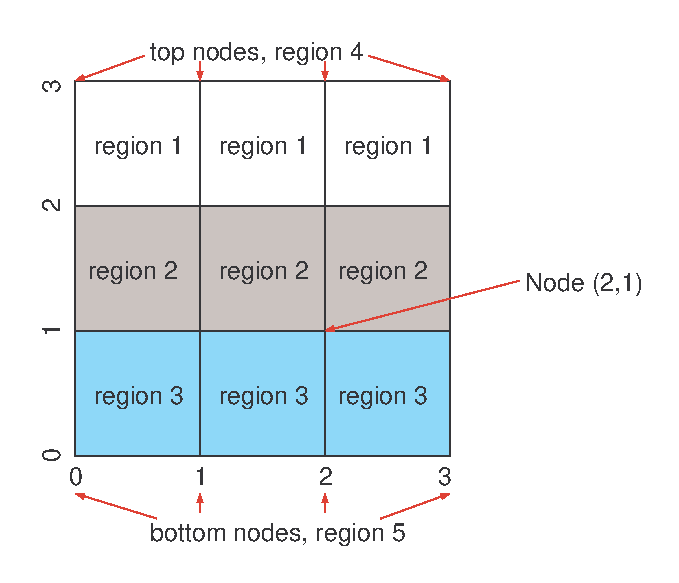
\includegraphics{mtfpic}
  \caption{2-D analogue of \zinc meshing.}
  \label{mtfpic}
\end{figure}
Consider the illustration \f{mtfpic}. Here the problem is shown in 2-D
for clarity. The 3-D mesh used in \zinc is analogous. In the figure, there are 3
material regions and we need to label the elements as region 1, 2 or 3
appropriately (we will later associate material properties with each
region). We want to label the top row of nodes as region 4 and the
bottom row as region 5. (We will later set Dirichlet boundaries for
nodes with region number 4 and 5). The region numbers of the internal
nodes does not matter provided it is not 4 or 5. Nodes with numbers 1,
2 or 3 will not be fixed. We will label internal nodes as 1. Note:
Metamesh will generally label the internal nodes the same as adjacent
elements as it performs the mesh.

Nodes are indexed as (0,0), (1,0) etc. Node (2,1) is indicated in the
figure. The complete zinc.mtf file would be:
\begin{verbatim}
IMax:  3
JMax:  3

 I    J    x    y    RegNo   RegUp
==================================
 0    0   0.0  0.0       5       3
 1    0   0.5  0.0       5       3
 2    0   etc...         5       3
 3    0                  5       0
 0    1                  1       2
 1    1                  1       2
 2    1                  1       2
 3    1                  1       0
 0    2                  1       1
 1    2                  1       1
 2    2                  1       1
 3    2                  1       0
 0    3                  4       0
 1    3                  4       0
 2    3                  4       0
 3    3                  4       0
\end{verbatim}
RegNo specifies the region number of the node in question. RegUp
specified the region number of the element connected to this node in
the positive I, J (and K for the 3-D case) direction.  Note that elements which do not
exists are labelled ``0''. 

Assuming one variable, the corresponding \var{filename.zin} file would be something like

\begin{verbatim}
region 1 elements 3 values C
1 1 1 1   2e-6
1 2 1 2   2e-6
1 3 1 3   2e-6

region 2 elements 4 values C
1 1 1 1   7e-6
1 1 1 2   4e-6
1 2 1 2   7e-6
1 3 1 3   7e-6

region 3 elements 6 values C
1 1 1 1   4e-6
1 2 1 2   4e-6
1 3 1 3   4e-6
1 1 1 2   3.6e-6
1 1 1 3   3.2e-6
1 3 1 3   7e-6

region 4 nodes 1 value
1 1.0

region 5 nodes 1 value
1 2.0
\end{verbatim}

\section{Storage of meshing information and solution}

Internally, \zinc\ stores the meshing in arrays \var{ireg, iregup,
  rnode}; and the current solution in \var{vec}. These are such that
(refering to \f{mtfpic}) \var{ireg(i,j,k)} is the region number of node \var{(i,j,k)};
\var{iregup(i,j,k)} is the region number of element \var{(i,j,k)}; and
\var{rnode(i,j,k,1)}, \var{rnode(i,j,k,2)}, \var{rnode(i,j,k,3)} 
are the (x,y,z) spatial coordinate (resp.) of node \var{(i,j,k)}.

The current solution for variable \var{ii} at node \var{(i,j,k)} is
stored in \var{vec(ind)} where
\begin{verbatim}
  ind=(k*(imax+1)*(jmax+1)+j*(imax+1)+i)*nvar+ii
\end{verbatim}
where \var{imax,jmax,kmax} are the extents of the meshing, with nodes
running from 0 to \var{imax} etc.

The variables \var{ireg, iregup, rnode, vec, imax, jmax, kmax} are passed through to
user-written functions \var{cfun} etc (see \sect{nonlin}) so the user has access to the
mesh geometry and current solution throughout the simulation. It is
expected that only advanced users will make use of these variables.

\chapter{Description of the \zinc\ ZOU ouptput file}
\label{zousec}

Here is an example of the file.
\begin{verbatim}
# Prepared by Zinc 3.4. Date: 25/04/2014. Time: 23:48:14

 istep=           1
    0    0    0    1   0.000000E+00
    0    0    0    2   0.111350E+06
    0    0    0    3   0.112150E+00
    0    0    0    4   0.000000E+00
    0    0    0    5   0.000000E+00
    0    0    0    6   0.000000E+00
    0    0    0    7   0.000000E+00
    0    0    0    8   0.000000E+00
    0    0    1    1   0.000000E+00
    0    0    1    2   0.111362E+06
    0    0    1    3   0.112153E+00
    0    0    1    4   0.000000E+00
    0    0    1    5   0.000000E+00
    0    0    1    6   0.000000E+00
    0    0    1    7   0.000000E+00
    0    0    1    8   0.000000E+00  
:

 (final) istep=   2
    0    0    0    1   0.000000E+00
    0    0    0    2   0.111350E+06
    0    0    0    3   0.112150E+00
    0    0    0    4   0.000000E+00
    0    0    0    5   0.000000E+00
    0    0    0    6   0.000000E+00
    0    0    0    7   0.000000E+00
    0    0    0    8   0.000000E+00
    0    0    1    1   0.000000E+00
    0    0    1    2   0.111362E+06
    0    0    1    3   0.112153E+00
    0    0    1    4   0.000000E+00
    0    0    1    5   0.000000E+00
    0    0    1    6   0.000000E+00
    0    0    1    7   0.000000E+00
    0    0    1    8   0.000000E+00  
\end{verbatim}
The first three columns are the node index (I,J,K) in the range
(0,IMAX-1), (0,JMAX-1), (0,KMAX-1). The fourth column is the variable
number (1,2,..nvar) and the fifth column gives the corresponding
solution value. In the case of static solutions there will be only one
snapshot in the file, for transient there are multiple snapshots with
the time for each snapshot indicated (istep) and the final snapshot
shown using ``(final)''. When restarting, transient simulations
continue from this final snapshot. For transient systems,
\zpp\ generates curves for each snapshot in the file.

The ZOU file can also appear in binary format depending on the
\var{zou\_format} command given in the ZIN file.

\chapter{Additional global variables in file.zin}
\label{additional}

These options are \emph{advanced} and should only be used by
developers or if you are feeling adventurous!

\begin{description}
\item[key\_db] 0: no debug info; 1: write debug info to \var{filename.zls}; 2:
  write detailed debug information. Create files showing shape of each
  element. (default 0)

\item[idmin, idbmax, jdbmin, jdbmax, kdbmin, kdbmax] range for
  elements (specified by lower nodes) to be written for debuging. Only
  used when key db=2

\item[key\_Q] 1: Build Q by node pairs (seems to be faster); 2 build Q
  by element (does not implement Surface commands); 3: use a tree
  structure to build Q (currently broken!); 4: assume all elements are
  cuboids aligned with the coordinate axes (much faster if true); 5:
  assume cuboid elements but build Q by element (default 1)

\item[nodecheck] YES: instead of writing the output solution, write a
  ZOU file where each degree of freedom is given a value specifying
  the type of boundary condition or constraint at that node. The
  values are: 1 deactivated (ie fixed at zero); 2 fixed at a non-zero
  value (including non-linear); 3 external Neumann boundary; 4
  internal Neumann boundary (bordering a void region); 5 continuity; 6
  variable (in the bulk). This file can be read into Zmesh in the
  usual way. Note that the solution is not output so you should run
  for zero iteration steps. (default=NO)
\end{description}

\end{document}
